% Options for packages loaded elsewhere
\PassOptionsToPackage{unicode}{hyperref}
\PassOptionsToPackage{hyphens}{url}
%
\documentclass[
]{article}
\usepackage{lmodern}
\usepackage{amssymb,amsmath}
\usepackage{ifxetex,ifluatex}
\ifnum 0\ifxetex 1\fi\ifluatex 1\fi=0 % if pdftex
  \usepackage[T1]{fontenc}
  \usepackage[utf8]{inputenc}
  \usepackage{textcomp} % provide euro and other symbols
\else % if luatex or xetex
  \usepackage{unicode-math}
  \defaultfontfeatures{Scale=MatchLowercase}
  \defaultfontfeatures[\rmfamily]{Ligatures=TeX,Scale=1}
\fi
% Use upquote if available, for straight quotes in verbatim environments
\IfFileExists{upquote.sty}{\usepackage{upquote}}{}
\IfFileExists{microtype.sty}{% use microtype if available
  \usepackage[]{microtype}
  \UseMicrotypeSet[protrusion]{basicmath} % disable protrusion for tt fonts
}{}
\makeatletter
\@ifundefined{KOMAClassName}{% if non-KOMA class
  \IfFileExists{parskip.sty}{%
    \usepackage{parskip}
  }{% else
    \setlength{\parindent}{0pt}
    \setlength{\parskip}{6pt plus 2pt minus 1pt}}
}{% if KOMA class
  \KOMAoptions{parskip=half}}
\makeatother
\usepackage{xcolor}
\IfFileExists{xurl.sty}{\usepackage{xurl}}{} % add URL line breaks if available
\IfFileExists{bookmark.sty}{\usepackage{bookmark}}{\usepackage{hyperref}}
\hypersetup{
  pdftitle={Double Lasso},
  hidelinks,
  pdfcreator={LaTeX via pandoc}}
\urlstyle{same} % disable monospaced font for URLs
\usepackage[margin=1in]{geometry}
\usepackage{color}
\usepackage{fancyvrb}
\newcommand{\VerbBar}{|}
\newcommand{\VERB}{\Verb[commandchars=\\\{\}]}
\DefineVerbatimEnvironment{Highlighting}{Verbatim}{commandchars=\\\{\}}
% Add ',fontsize=\small' for more characters per line
\usepackage{framed}
\definecolor{shadecolor}{RGB}{248,248,248}
\newenvironment{Shaded}{\begin{snugshade}}{\end{snugshade}}
\newcommand{\AlertTok}[1]{\textcolor[rgb]{0.94,0.16,0.16}{#1}}
\newcommand{\AnnotationTok}[1]{\textcolor[rgb]{0.56,0.35,0.01}{\textbf{\textit{#1}}}}
\newcommand{\AttributeTok}[1]{\textcolor[rgb]{0.77,0.63,0.00}{#1}}
\newcommand{\BaseNTok}[1]{\textcolor[rgb]{0.00,0.00,0.81}{#1}}
\newcommand{\BuiltInTok}[1]{#1}
\newcommand{\CharTok}[1]{\textcolor[rgb]{0.31,0.60,0.02}{#1}}
\newcommand{\CommentTok}[1]{\textcolor[rgb]{0.56,0.35,0.01}{\textit{#1}}}
\newcommand{\CommentVarTok}[1]{\textcolor[rgb]{0.56,0.35,0.01}{\textbf{\textit{#1}}}}
\newcommand{\ConstantTok}[1]{\textcolor[rgb]{0.00,0.00,0.00}{#1}}
\newcommand{\ControlFlowTok}[1]{\textcolor[rgb]{0.13,0.29,0.53}{\textbf{#1}}}
\newcommand{\DataTypeTok}[1]{\textcolor[rgb]{0.13,0.29,0.53}{#1}}
\newcommand{\DecValTok}[1]{\textcolor[rgb]{0.00,0.00,0.81}{#1}}
\newcommand{\DocumentationTok}[1]{\textcolor[rgb]{0.56,0.35,0.01}{\textbf{\textit{#1}}}}
\newcommand{\ErrorTok}[1]{\textcolor[rgb]{0.64,0.00,0.00}{\textbf{#1}}}
\newcommand{\ExtensionTok}[1]{#1}
\newcommand{\FloatTok}[1]{\textcolor[rgb]{0.00,0.00,0.81}{#1}}
\newcommand{\FunctionTok}[1]{\textcolor[rgb]{0.00,0.00,0.00}{#1}}
\newcommand{\ImportTok}[1]{#1}
\newcommand{\InformationTok}[1]{\textcolor[rgb]{0.56,0.35,0.01}{\textbf{\textit{#1}}}}
\newcommand{\KeywordTok}[1]{\textcolor[rgb]{0.13,0.29,0.53}{\textbf{#1}}}
\newcommand{\NormalTok}[1]{#1}
\newcommand{\OperatorTok}[1]{\textcolor[rgb]{0.81,0.36,0.00}{\textbf{#1}}}
\newcommand{\OtherTok}[1]{\textcolor[rgb]{0.56,0.35,0.01}{#1}}
\newcommand{\PreprocessorTok}[1]{\textcolor[rgb]{0.56,0.35,0.01}{\textit{#1}}}
\newcommand{\RegionMarkerTok}[1]{#1}
\newcommand{\SpecialCharTok}[1]{\textcolor[rgb]{0.00,0.00,0.00}{#1}}
\newcommand{\SpecialStringTok}[1]{\textcolor[rgb]{0.31,0.60,0.02}{#1}}
\newcommand{\StringTok}[1]{\textcolor[rgb]{0.31,0.60,0.02}{#1}}
\newcommand{\VariableTok}[1]{\textcolor[rgb]{0.00,0.00,0.00}{#1}}
\newcommand{\VerbatimStringTok}[1]{\textcolor[rgb]{0.31,0.60,0.02}{#1}}
\newcommand{\WarningTok}[1]{\textcolor[rgb]{0.56,0.35,0.01}{\textbf{\textit{#1}}}}
\usepackage{graphicx,grffile}
\makeatletter
\def\maxwidth{\ifdim\Gin@nat@width>\linewidth\linewidth\else\Gin@nat@width\fi}
\def\maxheight{\ifdim\Gin@nat@height>\textheight\textheight\else\Gin@nat@height\fi}
\makeatother
% Scale images if necessary, so that they will not overflow the page
% margins by default, and it is still possible to overwrite the defaults
% using explicit options in \includegraphics[width, height, ...]{}
\setkeys{Gin}{width=\maxwidth,height=\maxheight,keepaspectratio}
% Set default figure placement to htbp
\makeatletter
\def\fps@figure{htbp}
\makeatother
\setlength{\emergencystretch}{3em} % prevent overfull lines
\providecommand{\tightlist}{%
  \setlength{\itemsep}{0pt}\setlength{\parskip}{0pt}}
\setcounter{secnumdepth}{-\maxdimen} % remove section numbering

\title{Double Lasso}
\author{}
\date{\vspace{-2.5em}}

\begin{document}
\maketitle

\begin{Shaded}
\begin{Highlighting}[]
\NormalTok{knitr}\OperatorTok{::}\NormalTok{opts_chunk}\OperatorTok{$}\KeywordTok{set}\NormalTok{(}\DataTypeTok{echo =} \OtherTok{TRUE}\NormalTok{)}
\CommentTok{#+ setup, error=TRUE}
\end{Highlighting}
\end{Shaded}

\hypertarget{data-preparation}{%
\subsection{Data Preparation}\label{data-preparation}}

\begin{Shaded}
\begin{Highlighting}[]
\CommentTok{# Brian Kang}
\CommentTok{# Must use 64-bit version of R}
\CommentTok{#knitr::opts_chunk$set(error=TRUE)}
\CommentTok{#rm(list = ls())}

\KeywordTok{setwd}\NormalTok{(}\StringTok{"H:/Honors Research"}\NormalTok{)}
\CommentTok{#chooseCRANmirror(graphics=FALSE, ind=1)}
\CommentTok{#install.packages(c("hdm","dplyr","stringr","glmnet","gdata","fastDummies"))}
\KeywordTok{library}\NormalTok{(hdm)}
\KeywordTok{library}\NormalTok{(dplyr)}
\end{Highlighting}
\end{Shaded}

\begin{verbatim}
## 
## Attaching package: 'dplyr'
\end{verbatim}

\begin{verbatim}
## The following objects are masked from 'package:stats':
## 
##     filter, lag
\end{verbatim}

\begin{verbatim}
## The following objects are masked from 'package:base':
## 
##     intersect, setdiff, setequal, union
\end{verbatim}

\begin{Shaded}
\begin{Highlighting}[]
\KeywordTok{library}\NormalTok{(stringr)}
\KeywordTok{library}\NormalTok{(glmnet)}
\end{Highlighting}
\end{Shaded}

\begin{verbatim}
## Loading required package: Matrix
\end{verbatim}

\begin{verbatim}
## Loaded glmnet 3.0-2
\end{verbatim}

\begin{Shaded}
\begin{Highlighting}[]
\KeywordTok{library}\NormalTok{(gdata)}
\end{Highlighting}
\end{Shaded}

\begin{verbatim}
## gdata: Unable to locate valid perl interpreter
## gdata: 
## gdata: read.xls() will be unable to read Excel XLS and XLSX files
## gdata: unless the 'perl=' argument is used to specify the location of a
## gdata: valid perl intrpreter.
## gdata: 
## gdata: (To avoid display of this message in the future, please ensure
## gdata: perl is installed and available on the executable search path.)
\end{verbatim}

\begin{verbatim}
## gdata: Unable to load perl libaries needed by read.xls()
## gdata: to support 'XLX' (Excel 97-2004) files.
\end{verbatim}

\begin{verbatim}
## 
\end{verbatim}

\begin{verbatim}
## gdata: Unable to load perl libaries needed by read.xls()
## gdata: to support 'XLSX' (Excel 2007+) files.
\end{verbatim}

\begin{verbatim}
## 
\end{verbatim}

\begin{verbatim}
## gdata: Run the function 'installXLSXsupport()'
## gdata: to automatically download and install the perl
## gdata: libaries needed to support Excel XLS and XLSX formats.
\end{verbatim}

\begin{verbatim}
## 
## Attaching package: 'gdata'
\end{verbatim}

\begin{verbatim}
## The following objects are masked from 'package:dplyr':
## 
##     combine, first, last
\end{verbatim}

\begin{verbatim}
## The following object is masked from 'package:stats':
## 
##     nobs
\end{verbatim}

\begin{verbatim}
## The following object is masked from 'package:utils':
## 
##     object.size
\end{verbatim}

\begin{verbatim}
## The following object is masked from 'package:base':
## 
##     startsWith
\end{verbatim}

\begin{Shaded}
\begin{Highlighting}[]
\KeywordTok{library}\NormalTok{(fastDummies)}
\KeywordTok{library}\NormalTok{(lmtest)}
\end{Highlighting}
\end{Shaded}

\begin{verbatim}
## Loading required package: zoo
\end{verbatim}

\begin{verbatim}
## 
## Attaching package: 'zoo'
\end{verbatim}

\begin{verbatim}
## The following objects are masked from 'package:base':
## 
##     as.Date, as.Date.numeric
\end{verbatim}

\begin{Shaded}
\begin{Highlighting}[]
\KeywordTok{library}\NormalTok{(car)}
\end{Highlighting}
\end{Shaded}

\begin{verbatim}
## Loading required package: carData
\end{verbatim}

\begin{verbatim}
## 
## Attaching package: 'car'
\end{verbatim}

\begin{verbatim}
## The following object is masked from 'package:dplyr':
## 
##     recode
\end{verbatim}

\begin{Shaded}
\begin{Highlighting}[]
\CommentTok{#dat <- read.table("e20185wa0002000.txt", sep = ",")    # 5-year ACS survey Washington data}

\CommentTok{# Import dataset ---------------------------------------------------------------------------------------------------}
\NormalTok{temp <-}\StringTok{ }\KeywordTok{read.csv}\NormalTok{(}\StringTok{"psam_pusb.csv"}\NormalTok{, }\DataTypeTok{header =}\NormalTok{ T, }\DataTypeTok{nrows =} \DecValTok{1}\NormalTok{)}
\CommentTok{# columns that don't import as factors using default settings}
\NormalTok{fnf <-}\StringTok{ }\KeywordTok{c}\NormalTok{(}\StringTok{"DIVISION"}\NormalTok{,}\StringTok{"PUMA"}\NormalTok{,}\StringTok{"REGION"}\NormalTok{,}\StringTok{"ST"}\NormalTok{,}\StringTok{"ADJINC"}\NormalTok{,}\StringTok{"CIT"}\NormalTok{,}\StringTok{"COW"}\NormalTok{,}\StringTok{"DDRS"}\NormalTok{,}\StringTok{"DEAR"}\NormalTok{,}
         \StringTok{"DEYE"}\NormalTok{,}\StringTok{"DOUT"}\NormalTok{,}\StringTok{"DPHY"}\NormalTok{,}\StringTok{"DRAT"}\NormalTok{,}\StringTok{"DRATX"}\NormalTok{,}\StringTok{"DREM"}\NormalTok{,}\StringTok{"ENG"}\NormalTok{,}\StringTok{"FER"}\NormalTok{,}\StringTok{"GCL"}\NormalTok{,}\StringTok{"GCM"}\NormalTok{,}\StringTok{"GCR"}\NormalTok{,}
         \StringTok{"HINS1"}\NormalTok{,}\StringTok{"HINS2"}\NormalTok{,}\StringTok{"HINS3"}\NormalTok{,}\StringTok{"HINS4"}\NormalTok{,}\StringTok{"HINS5"}\NormalTok{,}\StringTok{"HINS6"}\NormalTok{,}\StringTok{"HINS7"}\NormalTok{,}\StringTok{"JWTR"}\NormalTok{,}\StringTok{"LANX"}\NormalTok{,}
         \StringTok{"MAR"}\NormalTok{,}\StringTok{"MARHD"}\NormalTok{,}\StringTok{"MARHM"}\NormalTok{,}\StringTok{"MARHT"}\NormalTok{,}\StringTok{"MARHW"}\NormalTok{,}\StringTok{"MIG"}\NormalTok{,}\StringTok{"MIL"}\NormalTok{,}\StringTok{"MLPA"}\NormalTok{,}\StringTok{"MLPB"}\NormalTok{,}\StringTok{"MLPCD"}\NormalTok{,}
         \StringTok{"MLPE"}\NormalTok{,}\StringTok{"MLPFG"}\NormalTok{,}\StringTok{"MLPH"}\NormalTok{,}\StringTok{"MLPI"}\NormalTok{,}\StringTok{"MLPJ"}\NormalTok{,}\StringTok{"MLPK"}\NormalTok{,}\StringTok{"NWAB"}\NormalTok{,}\StringTok{"NWAV"}\NormalTok{,}\StringTok{"NWLA"}\NormalTok{,}\StringTok{"NWLK"}\NormalTok{,}
         \StringTok{"NWRE"}\NormalTok{,}\StringTok{"RELP"}\NormalTok{,}\StringTok{"SCH"}\NormalTok{,}\StringTok{"SCHG"}\NormalTok{,}\StringTok{"SCHL"}\NormalTok{,}\StringTok{"SEX"}\NormalTok{,}\StringTok{"WKL"}\NormalTok{,}\StringTok{"WKW"}\NormalTok{,}\StringTok{"WRK"}\NormalTok{,}\StringTok{"ANC"}\NormalTok{,}\StringTok{"ANC1P"}\NormalTok{,}
         \StringTok{"ANC2P"}\NormalTok{,}\StringTok{"DECADE"}\NormalTok{,}\StringTok{"DIS"}\NormalTok{,}\StringTok{"DRIVESP"}\NormalTok{,}\StringTok{"ESP"}\NormalTok{,}\StringTok{"ESR"}\NormalTok{,}\StringTok{"FOD1P"}\NormalTok{,}\StringTok{"FOD2P"}\NormalTok{,}\StringTok{"HICOV"}\NormalTok{,}
         \StringTok{"HISP"}\NormalTok{,}\StringTok{"INDP"}\NormalTok{,}\StringTok{"JWAP"}\NormalTok{,}\StringTok{"JWDP"}\NormalTok{,}\StringTok{"LANP"}\NormalTok{,}\StringTok{"MIGPUMA"}\NormalTok{,}\StringTok{"MIGSP"}\NormalTok{,}\StringTok{"MSP"}\NormalTok{,}\StringTok{"NATIVITY"}\NormalTok{,}
         \StringTok{"NOP"}\NormalTok{,}\StringTok{"OC"}\NormalTok{,}\StringTok{"OCCP"}\NormalTok{,}\StringTok{"PAOC"}\NormalTok{,}\StringTok{"POBP"}\NormalTok{,}\StringTok{"POWPUMA"}\NormalTok{,}\StringTok{"POWSP"}\NormalTok{,}\StringTok{"PRIVCOV"}\NormalTok{,}\StringTok{"PUBCOV"}\NormalTok{,}
         \StringTok{"QTRBIR"}\NormalTok{,}\StringTok{"RAC1P"}\NormalTok{,}\StringTok{"RAC2P"}\NormalTok{,}\StringTok{"RAC3P"}\NormalTok{,}\StringTok{"RACAIAN"}\NormalTok{,}\StringTok{"RACASN"}\NormalTok{,}\StringTok{"RACBLK"}\NormalTok{,}\StringTok{"RACNH"}\NormalTok{,}
         \StringTok{"RACNUM"}\NormalTok{,}\StringTok{"RACPI"}\NormalTok{,}\StringTok{"RACSOR"}\NormalTok{,}\StringTok{"RACWHT"}\NormalTok{,}\StringTok{"RC"}\NormalTok{,}\StringTok{"SCIENGP"}\NormalTok{,}\StringTok{"SCIENGRLP"}\NormalTok{,}\StringTok{"SFN"}\NormalTok{,}
         \StringTok{"SFR"}\NormalTok{,}\StringTok{"VPS"}\NormalTok{,}\StringTok{"WAOB"}\NormalTok{)}
\CommentTok{# columns that do import as factors using default setting}
\NormalTok{fif <-}\StringTok{ }\KeywordTok{c}\NormalTok{(}\StringTok{"RT"}\NormalTok{,}\StringTok{"SERIALNO"}\NormalTok{,}\StringTok{"NAICSP"}\NormalTok{,}\StringTok{"SOCP"}\NormalTok{)}
\CommentTok{# all columns that are factors}
\NormalTok{fcf <-}\StringTok{ }\KeywordTok{append}\NormalTok{(fnf,fif)}
\NormalTok{fcf <-}\StringTok{ }\KeywordTok{append}\NormalTok{(fcf,}\KeywordTok{names}\NormalTok{(temp[,}\KeywordTok{c}\NormalTok{(}\DecValTok{131}\OperatorTok{:}\DecValTok{286}\NormalTok{)]))}
\CommentTok{# vector of classes of data columns}
\NormalTok{colclass <-}\StringTok{ }\KeywordTok{ifelse}\NormalTok{(}\KeywordTok{colnames}\NormalTok{(temp) }\OperatorTok\StringTok{ }\NormalTok{fcf, }\StringTok{'factor'}\NormalTok{, }\StringTok{'numeric'}\NormalTok{)}

\NormalTok{temp1 <-}\StringTok{ }\KeywordTok{read.csv}\NormalTok{(}\StringTok{"psam_pusa.csv"}\NormalTok{, }\DataTypeTok{header =}\NormalTok{ T, }\DataTypeTok{colClasses =}\NormalTok{ colclass)}
\NormalTok{temp2 <-}\StringTok{ }\KeywordTok{read.csv}\NormalTok{(}\StringTok{"psam_pusb.csv"}\NormalTok{, }\DataTypeTok{header =}\NormalTok{ T, }\DataTypeTok{colClasses =}\NormalTok{ colclass)}
\NormalTok{dat <-}\StringTok{ }\KeywordTok{rbind}\NormalTok{(temp1,temp2)}
\NormalTok{dat <-}\StringTok{ }\NormalTok{dat[,}\OperatorTok{-}\KeywordTok{c}\NormalTok{(}\DecValTok{1}\NormalTok{,}\DecValTok{2}\NormalTok{)] }\CommentTok{# drop unecessary IDs}
\NormalTok{dat <-}\StringTok{ }\NormalTok{dat[,}\OperatorTok{-}\KeywordTok{c}\NormalTok{(}\DecValTok{129}\OperatorTok{:}\DecValTok{284}\NormalTok{)] }\CommentTok{# drop unnecessary flag vars}

\CommentTok{# US Census: "Income used to calculate poverty status includes PERNP (earnings) and PINCP (income)"}

\CommentTok{# Calculate Income-Poverty ratio ----------------------------------------------------------------------------------}
\CommentTok{# (POVPIP only shows NA or <0.5 or >=0.5 so calculate actual ratio)}
\NormalTok{PovertyThreshold <-}\StringTok{ }\KeywordTok{rep}\NormalTok{(}\OtherTok{NA}\NormalTok{, }\KeywordTok{nrow}\NormalTok{(dat))}
\NormalTok{getThreshold <-}\StringTok{ }\ControlFlowTok{function}\NormalTok{(threshold) \{ }\CommentTok{# values from CPS 2018}
  \ControlFlowTok{for}\NormalTok{ (i }\ControlFlowTok{in} \DecValTok{1}\OperatorTok{:}\KeywordTok{nrow}\NormalTok{(dat)) \{}
    \ControlFlowTok{if}\NormalTok{ (dat}\OperatorTok{$}\NormalTok{AGEP[i] }\OperatorTok{<}\StringTok{ }\DecValTok{18}\NormalTok{) \{ }\CommentTok{# under 18 yrs}
\NormalTok{      threshold[i] <-}\StringTok{ }\OtherTok{NA}
\NormalTok{    \} }\ControlFlowTok{else} \ControlFlowTok{if}\NormalTok{ (dat}\OperatorTok{$}\NormalTok{SPORDER[i]}\OperatorTok{==}\DecValTok{1} \OperatorTok{&}\StringTok{ }\NormalTok{dat}\OperatorTok{$}\NormalTok{AGEP[i] }\OperatorTok{<}\StringTok{ }\DecValTok{65}\NormalTok{) \{ }\CommentTok{# individual}
\NormalTok{      threshold[i] <-}\StringTok{ }\DecValTok{13064}
\NormalTok{    \} }\ControlFlowTok{else} \ControlFlowTok{if}\NormalTok{ (dat}\OperatorTok{$}\NormalTok{SPORDER[i]}\OperatorTok{==}\DecValTok{1} \OperatorTok{&}\StringTok{ }\NormalTok{dat}\OperatorTok{$}\NormalTok{AGEP[i] }\OperatorTok{>=}\StringTok{ }\DecValTok{65}\NormalTok{) \{}
\NormalTok{      threshold[i] <-}\StringTok{ }\DecValTok{12043}
      \CommentTok{# AGEP doesn't have NA values}
\NormalTok{    \} }\ControlFlowTok{else} \ControlFlowTok{if}\NormalTok{ (dat}\OperatorTok{$}\NormalTok{SPORDER[i]}\OperatorTok{==}\DecValTok{2} \OperatorTok{&}\StringTok{ }\NormalTok{dat}\OperatorTok{$}\NormalTok{AGEP[i] }\OperatorTok{<}\StringTok{ }\DecValTok{65} \OperatorTok{&}\StringTok{ }\NormalTok{dat}\OperatorTok{$}\NormalTok{OC[i]}\OperatorTok{==}\DecValTok{0}\NormalTok{) \{ }\CommentTok{# two people}
\NormalTok{      threshold[i] <-}\StringTok{ }\DecValTok{16815}
\NormalTok{    \} }\ControlFlowTok{else} \ControlFlowTok{if}\NormalTok{ (dat}\OperatorTok{$}\NormalTok{SPORDER[i]}\OperatorTok{==}\DecValTok{2} \OperatorTok{&}\StringTok{ }\NormalTok{dat}\OperatorTok{$}\NormalTok{AGEP[i] }\OperatorTok{<}\StringTok{ }\DecValTok{65} \OperatorTok{&}\StringTok{ }\NormalTok{dat}\OperatorTok{$}\NormalTok{OC[i]}\OperatorTok{==}\DecValTok{1}\NormalTok{) \{}
\NormalTok{      threshold[i] <-}\StringTok{ }\DecValTok{17308}
\NormalTok{    \} }\ControlFlowTok{else} \ControlFlowTok{if}\NormalTok{ (dat}\OperatorTok{$}\NormalTok{SPORDER[i]}\OperatorTok{==}\DecValTok{2} \OperatorTok{&}\StringTok{ }\NormalTok{dat}\OperatorTok{$}\NormalTok{AGEP[i] }\OperatorTok{>=}\StringTok{ }\DecValTok{65} \OperatorTok{&}\StringTok{ }\NormalTok{dat}\OperatorTok{$}\NormalTok{OC[i]}\OperatorTok{==}\DecValTok{0}\NormalTok{) \{}
\NormalTok{      threshold[i] <-}\StringTok{ }\DecValTok{15178}
\NormalTok{    \} }\ControlFlowTok{else} \ControlFlowTok{if}\NormalTok{ (dat}\OperatorTok{$}\NormalTok{SPORDER[i]}\OperatorTok{==}\DecValTok{2} \OperatorTok{&}\StringTok{ }\NormalTok{dat}\OperatorTok{$}\NormalTok{AGEP[i] }\OperatorTok{>=}\StringTok{ }\DecValTok{65} \OperatorTok{&}\StringTok{ }\NormalTok{dat}\OperatorTok{$}\NormalTok{OC[i]}\OperatorTok{==}\DecValTok{1}\NormalTok{) \{}
\NormalTok{      threshold[i] <-}\StringTok{ }\DecValTok{17242}
\NormalTok{    \} }\ControlFlowTok{else} \ControlFlowTok{if}\NormalTok{ (dat}\OperatorTok{$}\NormalTok{SPORDER[i]}\OperatorTok{==}\DecValTok{2}\NormalTok{) \{ }\CommentTok{# OC is NA value}
\NormalTok{      threshold[i] <-}\StringTok{ }\DecValTok{16247}
\NormalTok{    \} }\ControlFlowTok{else} \ControlFlowTok{if}\NormalTok{ (dat}\OperatorTok{$}\NormalTok{SPORDER[i]}\OperatorTok{==}\DecValTok{3} \OperatorTok{&}\StringTok{ }\NormalTok{dat}\OperatorTok{$}\NormalTok{OC[i]}\OperatorTok{==}\DecValTok{0}\NormalTok{) \{ }\CommentTok{# three people}
\NormalTok{      threshold[i] <-}\StringTok{ }\DecValTok{19642}
\NormalTok{    \} }\ControlFlowTok{else} \ControlFlowTok{if}\NormalTok{ (dat}\OperatorTok{$}\NormalTok{SPORDER[i]}\OperatorTok{==}\DecValTok{3} \OperatorTok{&}\StringTok{ }\NormalTok{dat}\OperatorTok{$}\NormalTok{OC[i]}\OperatorTok{==}\DecValTok{1}\NormalTok{) \{}
\NormalTok{      threshold[i] <-}\StringTok{ }\NormalTok{(}\DecValTok{20212}\OperatorTok{+}\DecValTok{20231}\NormalTok{)}\OperatorTok{/}\DecValTok{2}
\NormalTok{    \} }\ControlFlowTok{else} \ControlFlowTok{if}\NormalTok{ (dat}\OperatorTok{$}\NormalTok{SPORDER[i]}\OperatorTok{==}\DecValTok{3}\NormalTok{) \{ }\CommentTok{# OC is NA value}
\NormalTok{      threshold[i] <-}\StringTok{ }\DecValTok{19985}
\NormalTok{    \} }\ControlFlowTok{else} \ControlFlowTok{if}\NormalTok{ (dat}\OperatorTok{$}\NormalTok{SPORDER[i]}\OperatorTok{==}\DecValTok{4} \OperatorTok{&}\StringTok{ }\NormalTok{dat}\OperatorTok{$}\NormalTok{OC[i]}\OperatorTok{==}\DecValTok{0}\NormalTok{) \{ }\CommentTok{# four people}
\NormalTok{      threshold[i] <-}\StringTok{ }\DecValTok{25900}
\NormalTok{    \} }\ControlFlowTok{else} \ControlFlowTok{if}\NormalTok{ (dat}\OperatorTok{$}\NormalTok{SPORDER[i]}\OperatorTok{==}\DecValTok{4} \OperatorTok{&}\StringTok{ }\NormalTok{dat}\OperatorTok{$}\NormalTok{OC[i]}\OperatorTok{==}\DecValTok{1}\NormalTok{) \{}
\NormalTok{      threshold[i] <-}\StringTok{ }\NormalTok{(}\DecValTok{26324}\OperatorTok{+}\DecValTok{25465}\OperatorTok{+}\DecValTok{25554}\NormalTok{)}\OperatorTok{/}\DecValTok{3}
\NormalTok{    \} }\ControlFlowTok{else} \ControlFlowTok{if}\NormalTok{ (dat}\OperatorTok{$}\NormalTok{SPORDER[i]}\OperatorTok{==}\DecValTok{4}\NormalTok{) \{ }\CommentTok{# OC is NA value}
\NormalTok{      threshold[i] <-}\StringTok{ }\DecValTok{25701}
\NormalTok{    \} }\ControlFlowTok{else} \ControlFlowTok{if}\NormalTok{ (dat}\OperatorTok{$}\NormalTok{SPORDER[i]}\OperatorTok{==}\DecValTok{5} \OperatorTok{&}\StringTok{ }\NormalTok{dat}\OperatorTok{$}\NormalTok{OC[i]}\OperatorTok{==}\DecValTok{0}\NormalTok{) \{ }\CommentTok{# five people}
\NormalTok{      threshold[i] <-}\StringTok{ }\DecValTok{31234}
\NormalTok{    \} }\ControlFlowTok{else} \ControlFlowTok{if}\NormalTok{ (dat}\OperatorTok{$}\NormalTok{SPORDER[i]}\OperatorTok{==}\DecValTok{5} \OperatorTok{&}\StringTok{ }\NormalTok{dat}\OperatorTok{$}\NormalTok{OC[i]}\OperatorTok{==}\DecValTok{1}\NormalTok{) \{}
\NormalTok{      threshold[i] <-}\StringTok{ }\NormalTok{(}\DecValTok{31689}\OperatorTok{+}\DecValTok{30718}\OperatorTok{+}\DecValTok{29967}\OperatorTok{+}\DecValTok{29509}\NormalTok{)}\OperatorTok{/}\DecValTok{4}
\NormalTok{    \} }\ControlFlowTok{else} \ControlFlowTok{if}\NormalTok{ (dat}\OperatorTok{$}\NormalTok{SPORDER[i]}\OperatorTok{==}\DecValTok{5}\NormalTok{) \{ }\CommentTok{# OC is NA value}
\NormalTok{      threshold[i] <-}\StringTok{ }\DecValTok{30459}
\NormalTok{    \} }\ControlFlowTok{else} \ControlFlowTok{if}\NormalTok{ (dat}\OperatorTok{$}\NormalTok{SPORDER[i]}\OperatorTok{==}\DecValTok{6} \OperatorTok{&}\StringTok{ }\NormalTok{dat}\OperatorTok{$}\NormalTok{OC[i]}\OperatorTok{==}\DecValTok{0}\NormalTok{) \{ }\CommentTok{# six people}
\NormalTok{      threshold[i] <-}\StringTok{ }\DecValTok{35925}
\NormalTok{    \} }\ControlFlowTok{else} \ControlFlowTok{if}\NormalTok{ (dat}\OperatorTok{$}\NormalTok{SPORDER[i]}\OperatorTok{==}\DecValTok{6} \OperatorTok{&}\StringTok{ }\NormalTok{dat}\OperatorTok{$}\NormalTok{OC[i]}\OperatorTok{==}\DecValTok{1}\NormalTok{) \{}
\NormalTok{      threshold[i] <-}\StringTok{ }\NormalTok{(}\DecValTok{36068}\OperatorTok{+}\DecValTok{35324}\OperatorTok{+}\DecValTok{34612}\OperatorTok{+}\DecValTok{33553}\OperatorTok{+}\DecValTok{32925}\NormalTok{)}\OperatorTok{/}\DecValTok{5}
\NormalTok{    \} }\ControlFlowTok{else} \ControlFlowTok{if}\NormalTok{ (dat}\OperatorTok{$}\NormalTok{SPORDER[i]}\OperatorTok{==}\DecValTok{6}\NormalTok{) \{ }\CommentTok{# OC is NA value}
\NormalTok{      threshold[i] <-}\StringTok{ }\DecValTok{34533}
\NormalTok{    \} }\ControlFlowTok{else} \ControlFlowTok{if}\NormalTok{ (dat}\OperatorTok{$}\NormalTok{SPORDER[i]}\OperatorTok{==}\DecValTok{7} \OperatorTok{&}\StringTok{ }\NormalTok{dat}\OperatorTok{$}\NormalTok{OC[i]}\OperatorTok{==}\DecValTok{0}\NormalTok{) \{ }\CommentTok{# seven people}
\NormalTok{      threshold[i] <-}\StringTok{ }\DecValTok{41336}
\NormalTok{    \} }\ControlFlowTok{else} \ControlFlowTok{if}\NormalTok{ (dat}\OperatorTok{$}\NormalTok{SPORDER[i]}\OperatorTok{==}\DecValTok{7} \OperatorTok{&}\StringTok{ }\NormalTok{dat}\OperatorTok{$}\NormalTok{OC[i]}\OperatorTok{==}\DecValTok{1}\NormalTok{) \{}
\NormalTok{      threshold[i] <-}\StringTok{ }\NormalTok{(}\DecValTok{4159}\OperatorTok{+}\DecValTok{40705}\OperatorTok{+}\DecValTok{40085}\OperatorTok{+}\DecValTok{38929}\OperatorTok{+}\DecValTok{37581}\OperatorTok{+}\DecValTok{36102}\NormalTok{)}\OperatorTok{/}\DecValTok{6}
\NormalTok{    \} }\ControlFlowTok{else} \ControlFlowTok{if}\NormalTok{ (dat}\OperatorTok{$}\NormalTok{SPORDER[i]}\OperatorTok{==}\DecValTok{7}\NormalTok{) \{ }\CommentTok{# OC is NA value}
\NormalTok{      threshold[i] <-}\StringTok{ }\DecValTok{39194}
\NormalTok{    \} }\ControlFlowTok{else} \ControlFlowTok{if}\NormalTok{ (dat}\OperatorTok{$}\NormalTok{SPORDER[i]}\OperatorTok{==}\DecValTok{8} \OperatorTok{&}\StringTok{ }\NormalTok{dat}\OperatorTok{$}\NormalTok{OC[i]}\OperatorTok{==}\DecValTok{0}\NormalTok{) \{ }\CommentTok{# eight people}
\NormalTok{      threshold[i] <-}\StringTok{ }\DecValTok{46231}
\NormalTok{    \} }\ControlFlowTok{else} \ControlFlowTok{if}\NormalTok{ (dat}\OperatorTok{$}\NormalTok{SPORDER[i]}\OperatorTok{==}\DecValTok{8} \OperatorTok{&}\StringTok{ }\NormalTok{dat}\OperatorTok{$}\NormalTok{OC[i]}\OperatorTok{==}\DecValTok{1}\NormalTok{) \{}
\NormalTok{      threshold[i] <-}\StringTok{ }\NormalTok{(}\DecValTok{46640}\OperatorTok{+}\DecValTok{45800}\OperatorTok{+}\DecValTok{45064}\OperatorTok{+}\DecValTok{44021}\OperatorTok{+}\DecValTok{42696}\OperatorTok{+}\DecValTok{41317}\OperatorTok{+}\DecValTok{40967}\NormalTok{)}\OperatorTok{/}\DecValTok{7}
\NormalTok{    \} }\ControlFlowTok{else} \ControlFlowTok{if}\NormalTok{ (dat}\OperatorTok{$}\NormalTok{SPORDER[i]}\OperatorTok{==}\DecValTok{8}\NormalTok{) \{ }\CommentTok{# OC is NA value}
\NormalTok{      threshold[i] <-}\StringTok{ }\DecValTok{43602}
\NormalTok{    \} }\ControlFlowTok{else} \ControlFlowTok{if}\NormalTok{ (dat}\OperatorTok{$}\NormalTok{SPORDER[i]}\OperatorTok{>=}\DecValTok{9} \OperatorTok{&}\StringTok{ }\NormalTok{dat}\OperatorTok{$}\NormalTok{OC[i]}\OperatorTok{==}\DecValTok{0}\NormalTok{) \{ }\CommentTok{# nine or more people}
\NormalTok{      threshold[i] <-}\StringTok{ }\DecValTok{55613}
\NormalTok{    \} }\ControlFlowTok{else} \ControlFlowTok{if}\NormalTok{ (dat}\OperatorTok{$}\NormalTok{SPORDER[i]}\OperatorTok{>=}\DecValTok{9} \OperatorTok{&}\StringTok{ }\NormalTok{dat}\OperatorTok{$}\NormalTok{OC[i]}\OperatorTok{==}\DecValTok{1}\NormalTok{) \{}
\NormalTok{      threshold[i] <-}\StringTok{ }\NormalTok{(}\DecValTok{55883}\OperatorTok{+}\DecValTok{55140}\OperatorTok{+}\DecValTok{54516}\OperatorTok{+}\DecValTok{53491}\OperatorTok{+}\DecValTok{52082}\OperatorTok{+}\DecValTok{50807}\OperatorTok{+}\DecValTok{50491}\OperatorTok{+}\DecValTok{48546}\NormalTok{)}\OperatorTok{/}\DecValTok{8}
\NormalTok{    \} }\ControlFlowTok{else} \ControlFlowTok{if}\NormalTok{ (dat}\OperatorTok{$}\NormalTok{SPORDER[i]}\OperatorTok{>=}\DecValTok{9}\NormalTok{) \{ }\CommentTok{# OC is NA value}
\NormalTok{      threshold[i] <-}\StringTok{ }\DecValTok{51393}
\NormalTok{    \} }\ControlFlowTok{else}\NormalTok{ \{}
\NormalTok{      threshold[i] <-}\StringTok{ }\OtherTok{NA}
\NormalTok{    \}}
\NormalTok{  \} }\CommentTok{# individually assign poverty threshold}
  \KeywordTok{return}\NormalTok{(threshold)}
\NormalTok{\}}
\NormalTok{PovertyThreshold <-}\StringTok{ }\KeywordTok{getThreshold}\NormalTok{(PovertyThreshold)}
\NormalTok{dat}\OperatorTok{$}\NormalTok{IncomePovertyRatio <-}\StringTok{ }\NormalTok{(dat}\OperatorTok{$}\NormalTok{PERNP }\OperatorTok{+}\StringTok{ }\NormalTok{dat}\OperatorTok{$}\NormalTok{PINCP)}\OperatorTok{/}\NormalTok{PovertyThreshold}
\NormalTok{dat}\OperatorTok{$}\NormalTok{IncomePovertyRatio <-}\StringTok{ }\NormalTok{dat}\OperatorTok{$}\NormalTok{IncomePovertyRatio }\OperatorTok{+}\StringTok{ }\DecValTok{1} \OperatorTok{+}\StringTok{ }\KeywordTok{abs}\NormalTok{(}\KeywordTok{min}\NormalTok{(dat}\OperatorTok{$}\NormalTok{IncomePovertyRatio, }\DataTypeTok{na.rm=}\NormalTok{na.omit)) }\CommentTok{# ensure all values are positive}


\CommentTok{# function for catching error in rlasso}
\NormalTok{myTryCatch <-}\StringTok{ }\ControlFlowTok{function}\NormalTok{(expr) \{}
\NormalTok{  warn <-}\StringTok{ }\NormalTok{err <-}\StringTok{ }\OtherTok{NULL}
\NormalTok{  value <-}\StringTok{ }\KeywordTok{withCallingHandlers}\NormalTok{(}
    \KeywordTok{tryCatch}\NormalTok{(expr, }\DataTypeTok{error=}\ControlFlowTok{function}\NormalTok{(e) \{}
\NormalTok{      err <<-}\StringTok{ }\NormalTok{e}
      \OtherTok{NULL}
\NormalTok{    \}), }\DataTypeTok{warning=}\ControlFlowTok{function}\NormalTok{(w) \{}
\NormalTok{      warn <<-}\StringTok{ }\NormalTok{w}
      \KeywordTok{invokeRestart}\NormalTok{(}\StringTok{"muffleWarning"}\NormalTok{)}
\NormalTok{    \})}
  \KeywordTok{list}\NormalTok{(}\DataTypeTok{error=}\NormalTok{err)}
\NormalTok{\}}
\end{Highlighting}
\end{Shaded}

\hypertarget{endogenous-double-ml}{%
\subsection{Endogenous Double ML}\label{endogenous-double-ml}}

\begin{Shaded}
\begin{Highlighting}[]
\CommentTok{## Initial Model 2: Double ML (Double LASSO) ----------------------------------------------------------------}
\NormalTok{temp <-}\StringTok{ }\NormalTok{dat}
\NormalTok{dat <-}\StringTok{ }\NormalTok{temp }\CommentTok{# recover original dataset}

\CommentTok{# DATA CLEANING FOR DOUBLE LASSO}
\NormalTok{nums <-}\StringTok{ }\KeywordTok{unlist}\NormalTok{(}\KeywordTok{lapply}\NormalTok{(dat, is.factor))}
\NormalTok{dattemp <-}\StringTok{ }\NormalTok{dat[,nums] }\CommentTok{# all the factors of dataset}
\CommentTok{# delete variables have >51 factor levels}
\NormalTok{get1 <-}\StringTok{ }\KeywordTok{names}\NormalTok{(}\KeywordTok{which}\NormalTok{(}\KeywordTok{sapply}\NormalTok{(dattemp, }\ControlFlowTok{function}\NormalTok{(x) }\KeywordTok{length}\NormalTok{(}\KeywordTok{unique}\NormalTok{(x))}\OperatorTok{>}\DecValTok{51}\NormalTok{)))}
\NormalTok{delete <-}\StringTok{ }\KeywordTok{which}\NormalTok{(}\KeywordTok{names}\NormalTok{(dat) }\OperatorTok\StringTok{ }\NormalTok{get1[}\OperatorTok{-}\DecValTok{16}\NormalTok{])}
\NormalTok{dat <-}\StringTok{ }\NormalTok{dat[,}\OperatorTok{-}\KeywordTok{c}\NormalTok{(delete)]}
\NormalTok{dat <-}\StringTok{ }\NormalTok{dat[,}\OperatorTok{-}\KeywordTok{c}\NormalTok{(}\DecValTok{9}\NormalTok{,}\DecValTok{43}\OperatorTok{:}\DecValTok{52}\NormalTok{,}\DecValTok{82}\NormalTok{,}\DecValTok{90}\NormalTok{,}\DecValTok{108}\NormalTok{,}\DecValTok{95}\NormalTok{,}\DecValTok{100}\NormalTok{)] }\CommentTok{# delete CITWP,MIL~MLPK,HISP,POVPIP,SFR,RAC1P,RACNUM}
\NormalTok{dat <-}\StringTok{ }\NormalTok{dat[,}\OperatorTok{-}\KeywordTok{c}\NormalTok{(}\DecValTok{1}\NormalTok{,}\DecValTok{3}\NormalTok{,}\DecValTok{76}\NormalTok{,}\DecValTok{77}\NormalTok{)] }\CommentTok{# delete DIVISION,REGION,PERNP,PINCP}
\CommentTok{# delete NA rows for Income-Poverty ratio}
\NormalTok{dat <-}\StringTok{ }\NormalTok{dat[}\OperatorTok{!}\KeywordTok{is.na}\NormalTok{(dat}\OperatorTok{$}\NormalTok{IncomePovertyRatio),]}
\NormalTok{dat <-}\StringTok{ }\NormalTok{dat[,}\OperatorTok{-}\KeywordTok{c}\NormalTok{(}\KeywordTok{which}\NormalTok{(}\KeywordTok{colnames}\NormalTok{(dat)}\OperatorTok{==}\StringTok{"JWRIP"}\NormalTok{),}\KeywordTok{which}\NormalTok{(}\KeywordTok{colnames}\NormalTok{(dat)}\OperatorTok{==}\StringTok{"YOEP"}\NormalTok{))]}
\CommentTok{# delete NA rows for JWMNP (travel time to work)}
\NormalTok{dat <-}\StringTok{ }\NormalTok{dat[}\OperatorTok{!}\KeywordTok{is.na}\NormalTok{(dat}\OperatorTok{$}\NormalTok{JWMNP),]}
\CommentTok{# delete NA rows for MARHYP: for factor <2 error}
\NormalTok{dat <-}\StringTok{ }\NormalTok{dat[}\OperatorTok{!}\KeywordTok{is.na}\NormalTok{(dat}\OperatorTok{$}\NormalTok{MARHYP),]}
\CommentTok{# delete NA rows for WKHP (usual hours worked per week)}
\NormalTok{dat <-}\StringTok{ }\NormalTok{dat[}\OperatorTok{!}\KeywordTok{is.na}\NormalTok{(dat}\OperatorTok{$}\NormalTok{WKHP),]}

\CommentTok{# delete/add vars that should be deleted/added (from correlation/causal inference)}
\NormalTok{dat <-}\StringTok{ }\NormalTok{dat[, }\OperatorTok{-}\KeywordTok{which}\NormalTok{(}\KeywordTok{names}\NormalTok{(dat) }\OperatorTok\StringTok{ }\KeywordTok{c}\NormalTok{(}\StringTok{"INTP"}\NormalTok{,}\StringTok{"OIP"}\NormalTok{,}\StringTok{"PAP"}\NormalTok{,}\StringTok{"RETP"}\NormalTok{,}\StringTok{"SEMP"}\NormalTok{,}\StringTok{"SSIP"}\NormalTok{,}\StringTok{"SSP"}\NormalTok{,}\StringTok{"WAGP"}\NormalTok{))]   }\CommentTok{# drop values related to Income}
\NormalTok{dat <-}\StringTok{ }\NormalTok{dat[, }\OperatorTok{-}\KeywordTok{which}\NormalTok{(}\KeywordTok{names}\NormalTok{(dat) }\OperatorTok\StringTok{ }\KeywordTok{c}\NormalTok{(}\StringTok{"SCH"}\NormalTok{,}\StringTok{"SCHG"}\NormalTok{))]   }\CommentTok{# drop weird educ vars}
\NormalTok{dat <-}\StringTok{ }\NormalTok{dat[, }\OperatorTok{-}\KeywordTok{which}\NormalTok{(}\KeywordTok{names}\NormalTok{(dat) }\OperatorTok\StringTok{ }\KeywordTok{c}\NormalTok{(}\StringTok{"ANC"}\NormalTok{))]  }\CommentTok{# drop ancestry}
\NormalTok{dat <-}\StringTok{ }\KeywordTok{droplevels}\NormalTok{(dat)}
\NormalTok{dat <-}\StringTok{ }\NormalTok{dat[, }\OperatorTok{-}\KeywordTok{which}\NormalTok{(}\KeywordTok{names}\NormalTok{(dat) }\OperatorTok\StringTok{ }\KeywordTok{c}\NormalTok{(}\StringTok{"ESR"}\NormalTok{,}\StringTok{"ESP"}\NormalTok{))]  }\CommentTok{# drop meaningless labor vars}
\NormalTok{dat <-}\StringTok{ }\NormalTok{dat[, }\OperatorTok{-}\KeywordTok{which}\NormalTok{(}\KeywordTok{names}\NormalTok{(dat) }\OperatorTok\StringTok{ }\KeywordTok{c}\NormalTok{(}\StringTok{"HICOV"}\NormalTok{,}\StringTok{"PRIVCOV"}\NormalTok{,}\StringTok{"PUBCOV"}\NormalTok{))]  }\CommentTok{# drop redundant insurance vars}
\NormalTok{dat <-}\StringTok{ }\NormalTok{dat[, }\OperatorTok{-}\KeywordTok{which}\NormalTok{(}\KeywordTok{names}\NormalTok{(dat) }\OperatorTok\StringTok{ }\KeywordTok{c}\NormalTok{(}\StringTok{"OC"}\NormalTok{,}\StringTok{"RC"}\NormalTok{))]  }\CommentTok{# drop child vars. Lack data}
\NormalTok{dat <-}\StringTok{ }\NormalTok{dat[, }\OperatorTok{-}\KeywordTok{which}\NormalTok{(}\KeywordTok{names}\NormalTok{(dat) }\OperatorTok\StringTok{ }\KeywordTok{c}\NormalTok{(}\StringTok{"SFN"}\NormalTok{))]  }\CommentTok{# drop "subfamily number"}
\NormalTok{dat <-}\StringTok{ }\NormalTok{dat[, }\OperatorTok{-}\KeywordTok{which}\NormalTok{(}\KeywordTok{names}\NormalTok{(dat) }\OperatorTok\StringTok{ }\KeywordTok{c}\NormalTok{(}\StringTok{"WRK"}\NormalTok{))]  }\CommentTok{# drop "worked last week" (we don't know when is "last week")}

\NormalTok{dat <-}\StringTok{ }\KeywordTok{cbind}\NormalTok{(dat, }\KeywordTok{model.matrix}\NormalTok{(}\OperatorTok{~}\NormalTok{(AGEP}\OperatorTok{:}\NormalTok{HINS3), dat)[,}\OperatorTok{-}\DecValTok{1}\NormalTok{])  }\CommentTok{# age*medicare}
\NormalTok{dat <-}\StringTok{ }\KeywordTok{cbind}\NormalTok{(dat, }\KeywordTok{model.matrix}\NormalTok{(}\OperatorTok{~}\NormalTok{(SCIENGP}\OperatorTok{:}\NormalTok{SCHL), dat)[,}\OperatorTok{-}\DecValTok{1}\NormalTok{])  }\CommentTok{# stem degree*attained degree}
\NormalTok{dat <-}\StringTok{ }\KeywordTok{cbind}\NormalTok{(dat, }\KeywordTok{model.matrix}\NormalTok{(}\OperatorTok{~}\NormalTok{(SCIENGRLP}\OperatorTok{:}\NormalTok{SCHL), dat)[,}\OperatorTok{-}\DecValTok{1}\NormalTok{])  }\CommentTok{# stem related degree*attained degree}
\NormalTok{dat}\OperatorTok{$}\NormalTok{VETERAN <-}\StringTok{ }\KeywordTok{ifelse}\NormalTok{((dat}\OperatorTok{$}\NormalTok{DRATX }\OperatorTok\StringTok{ }\KeywordTok{c}\NormalTok{(}\StringTok{"1"}\NormalTok{,}\StringTok{"2"}\NormalTok{)), }\DecValTok{1}\NormalTok{, }\DecValTok{0}\NormalTok{)  }\CommentTok{# veteran or not}
\NormalTok{dat <-}\StringTok{ }\NormalTok{dat[, }\OperatorTok{-}\KeywordTok{which}\NormalTok{(}\KeywordTok{names}\NormalTok{(dat) }\OperatorTok\StringTok{ }\KeywordTok{c}\NormalTok{(}\StringTok{"DRATX"}\NormalTok{,}\StringTok{"VPS"}\NormalTok{,}\StringTok{"DRAT"}\NormalTok{))]  }\CommentTok{# drop veteran related vars}
\NormalTok{dat <-}\StringTok{ }\KeywordTok{cbind}\NormalTok{(dat, }\KeywordTok{model.matrix}\NormalTok{(}\OperatorTok{~}\NormalTok{(AGEP}\OperatorTok{:}\NormalTok{VETERAN), dat)[,}\DecValTok{2}\NormalTok{])  }\CommentTok{# age*veteran or not}
\KeywordTok{names}\NormalTok{(dat)[}\KeywordTok{ncol}\NormalTok{(dat)] <-}\StringTok{ "AGEP_VETERAN"}
\NormalTok{dat <-}\StringTok{ }\KeywordTok{cbind}\NormalTok{(dat, }\KeywordTok{model.matrix}\NormalTok{(}\OperatorTok{~}\NormalTok{(AGEP}\OperatorTok{:}\NormalTok{GCL), dat)[,}\OperatorTok{-}\DecValTok{1}\NormalTok{])  }\CommentTok{# age*grandparent living with grandchild}
\NormalTok{dat <-}\StringTok{ }\KeywordTok{cbind}\NormalTok{(dat, }\KeywordTok{model.matrix}\NormalTok{(}\OperatorTok{~}\NormalTok{(AGEP}\OperatorTok{:}\NormalTok{GCR), dat)[,}\OperatorTok{-}\DecValTok{1}\NormalTok{])  }\CommentTok{# age*grandparent responsible grandchild}

\CommentTok{# logical dummy for ST==POWSP: most are FALSE}
\NormalTok{dat}\OperatorTok{$}\NormalTok{SameResidenceWorkplace <-}\StringTok{ }\NormalTok{(}\KeywordTok{as.numeric}\NormalTok{(dat}\OperatorTok{$}\NormalTok{ST)}\OperatorTok{==}\KeywordTok{as.numeric}\NormalTok{(dat}\OperatorTok{$}\NormalTok{POWSP))}
\NormalTok{dat <-}\StringTok{ }\NormalTok{dat[,}\OperatorTok{-}\KeywordTok{which}\NormalTok{(}\KeywordTok{names}\NormalTok{(dat) }\OperatorTok\StringTok{ }\KeywordTok{c}\NormalTok{(}\StringTok{"ST"}\NormalTok{,}\StringTok{"POWSP"}\NormalTok{))]  }\CommentTok{# delete ST,POWSP}
\CommentTok{# get which variables have <2 factor levels}
\NormalTok{get2 <-}\StringTok{ }\KeywordTok{which}\NormalTok{(}\KeywordTok{sapply}\NormalTok{(dat, }\ControlFlowTok{function}\NormalTok{(x) }\KeywordTok{length}\NormalTok{(}\KeywordTok{unique}\NormalTok{(x)))}\OperatorTok{<}\DecValTok{2}\NormalTok{)}
\NormalTok{dat <-}\StringTok{ }\NormalTok{dat[,}\OperatorTok{-}\NormalTok{get2]}
\KeywordTok{names}\NormalTok{(dat) <-}\StringTok{ }\KeywordTok{str_replace}\NormalTok{(}\KeywordTok{names}\NormalTok{(dat), }\StringTok{":"}\NormalTok{, }\StringTok{"_"}\NormalTok{) }\CommentTok{# reformat interaction term names}

\CommentTok{# STEP 1: FIRST LASSO: LOG(IncPovRatio) on ALL POTENTIAL VARIATES (i.e. y on focals)}
\NormalTok{varnames <-}\StringTok{ }\KeywordTok{paste}\NormalTok{(}\KeywordTok{c}\NormalTok{(}\KeywordTok{names}\NormalTok{(dat[,}\OperatorTok{-}\KeywordTok{c}\NormalTok{(}\KeywordTok{which}\NormalTok{(}\KeywordTok{names}\NormalTok{(dat) }\OperatorTok\StringTok{ }
\StringTok{                                          }\KeywordTok{c}\NormalTok{(}\StringTok{"IncomePovertyRatio"}\NormalTok{,}\StringTok{"SameResidenceWorkplace"}\NormalTok{,}
                                            \StringTok{"JWMNP"}\NormalTok{,}\StringTok{"JWTR"}\NormalTok{)))])), }\DataTypeTok{collapse =} \StringTok{"+"}\NormalTok{)}
\CommentTok{# throw in everything and see what happens with this LASSO}
\NormalTok{formula <-}\StringTok{ }\KeywordTok{paste}\NormalTok{(}\KeywordTok{c}\NormalTok{(}\StringTok{"log(IncomePovertyRatio)"}\NormalTok{,varnames), }\DataTypeTok{collapse =} \StringTok{"~"}\NormalTok{)}

\CommentTok{# Split data into train and test for K-fold CV}
\KeywordTok{set.seed}\NormalTok{(}\DecValTok{497}\NormalTok{)}
\NormalTok{train <-}\StringTok{ }\KeywordTok{sample}\NormalTok{(}\DecValTok{1}\OperatorTok{:}\KeywordTok{nrow}\NormalTok{(dat), }\KeywordTok{nrow}\NormalTok{(dat)}\OperatorTok{*}\FloatTok{0.8}\NormalTok{)  }\CommentTok{# 80% for training}

\CommentTok{# get which variables have <2 factor levels AFTER SUBSETTING}
\NormalTok{get <-}\StringTok{ }\KeywordTok{which}\NormalTok{(}\KeywordTok{sapply}\NormalTok{(dat[train,], }\ControlFlowTok{function}\NormalTok{(x) }\KeywordTok{length}\NormalTok{(}\KeywordTok{unique}\NormalTok{(x))}\OperatorTok{<}\DecValTok{2}\NormalTok{))}

\CommentTok{# get train and test datasets}
\CommentTok{# takeout intercept}
\NormalTok{xtrain <-}\StringTok{ }\KeywordTok{model.matrix}\NormalTok{(}\KeywordTok{as.formula}\NormalTok{(formula), }\DataTypeTok{data =}\NormalTok{ dat[train,])[,}\OperatorTok{-}\DecValTok{1}\NormalTok{]}
\NormalTok{ytrain <-}\StringTok{ }\KeywordTok{log}\NormalTok{(dat[train,]}\OperatorTok{$}\NormalTok{IncomePovertyRatio)}

\CommentTok{# cross validation then fit LASSO}
\NormalTok{cv.lasso}\FloatTok{.1}\NormalTok{ <-}\StringTok{ }\KeywordTok{cv.glmnet}\NormalTok{(xtrain, ytrain, }\DataTypeTok{alpha =} \DecValTok{1}\NormalTok{)  }\CommentTok{# 1 for lasso}
\NormalTok{cv.lambda}\FloatTok{.1}\NormalTok{ <-}\StringTok{ }\NormalTok{cv.lasso}\FloatTok{.1}\OperatorTok{$}\NormalTok{lambda.min  }\CommentTok{# get smallest tuning parameter}
\NormalTok{cv.lambda}\FloatTok{.1}
\end{Highlighting}
\end{Shaded}

\begin{verbatim}
## [1] 0.0001775132
\end{verbatim}

\begin{Shaded}
\begin{Highlighting}[]
\KeywordTok{plot}\NormalTok{(cv.lasso}\FloatTok{.1}\NormalTok{)}
\end{Highlighting}
\end{Shaded}

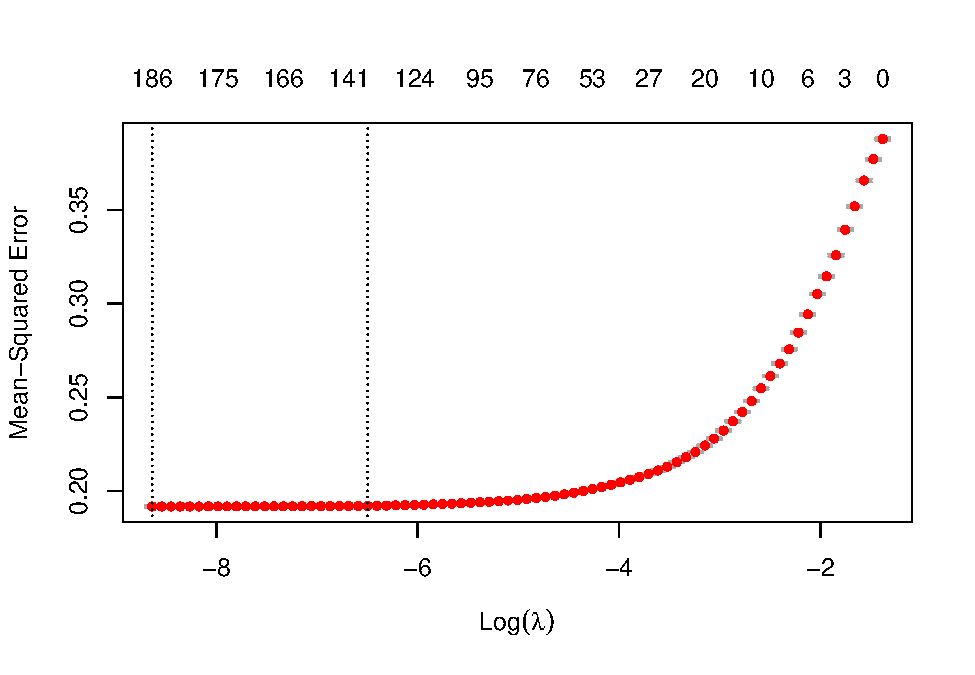
\includegraphics{dlassoMarkdown_files/figure-latex/unnamed-chunk-2-1.pdf}

\begin{Shaded}
\begin{Highlighting}[]
\CommentTok{# run lasso and get the necessary focal variables}
\NormalTok{dlasso}\FloatTok{.1}\NormalTok{ <-}\StringTok{ }\KeywordTok{rlasso}\NormalTok{(formula, }\DataTypeTok{data =}\NormalTok{ dat[train,], }
                   \DataTypeTok{lambda.start =}\NormalTok{ cv.lambda}\FloatTok{.1}\NormalTok{, }\DataTypeTok{post =}\NormalTok{ F)}
\CommentTok{#summary(lasso.2, all = F)}
\NormalTok{control <-}\StringTok{ }\KeywordTok{which}\NormalTok{(}\KeywordTok{coef}\NormalTok{(dlasso}\FloatTok{.1}\NormalTok{)[}\OperatorTok{-}\DecValTok{1}\NormalTok{]}\OperatorTok{!=}\DecValTok{0}\NormalTok{)}
\KeywordTok{length}\NormalTok{(control)}
\end{Highlighting}
\end{Shaded}

\begin{verbatim}
## [1] 157
\end{verbatim}

\begin{Shaded}
\begin{Highlighting}[]
\CommentTok{# STEP 2: SECOND LASSO: Core vars on ALL POTENTIAL VARIATES (i.e. focal on controls)}
\NormalTok{formula2}\FloatTok{.1}\NormalTok{ <-}\StringTok{ }\KeywordTok{paste}\NormalTok{(}\KeywordTok{c}\NormalTok{(}\StringTok{"SameResidenceWorkplace"}\NormalTok{,varnames), }\DataTypeTok{collapse =} \StringTok{"~"}\NormalTok{)}
\CommentTok{# k-fold cv}
\NormalTok{xtrain <-}\StringTok{ }\KeywordTok{model.matrix}\NormalTok{(}\KeywordTok{as.formula}\NormalTok{(formula2}\FloatTok{.1}\NormalTok{), }\DataTypeTok{data =}\NormalTok{ dat[train,])[,}\OperatorTok{-}\DecValTok{1}\NormalTok{]}
\NormalTok{ytrain <-}\StringTok{ }\NormalTok{dat[train,]}\OperatorTok{$}\NormalTok{SameResidenceWorkplace}
\NormalTok{cv.lasso.}\FloatTok{2.1}\NormalTok{ <-}\StringTok{ }\KeywordTok{cv.glmnet}\NormalTok{(xtrain, ytrain, }\DataTypeTok{alpha =} \DecValTok{1}\NormalTok{)  }\CommentTok{# 1 for lasso}
\NormalTok{cv.lambda.}\FloatTok{2.1}\NormalTok{ <-}\StringTok{ }\NormalTok{cv.lasso.}\FloatTok{2.1}\OperatorTok{$}\NormalTok{lambda.min  }\CommentTok{# get smallest tuning parameter}
\NormalTok{cv.lambda.}\FloatTok{2.1}
\end{Highlighting}
\end{Shaded}

\begin{verbatim}
## [1] 6.405355e-05
\end{verbatim}

\begin{Shaded}
\begin{Highlighting}[]
\KeywordTok{plot}\NormalTok{(cv.lasso.}\FloatTok{2.1}\NormalTok{)}
\end{Highlighting}
\end{Shaded}

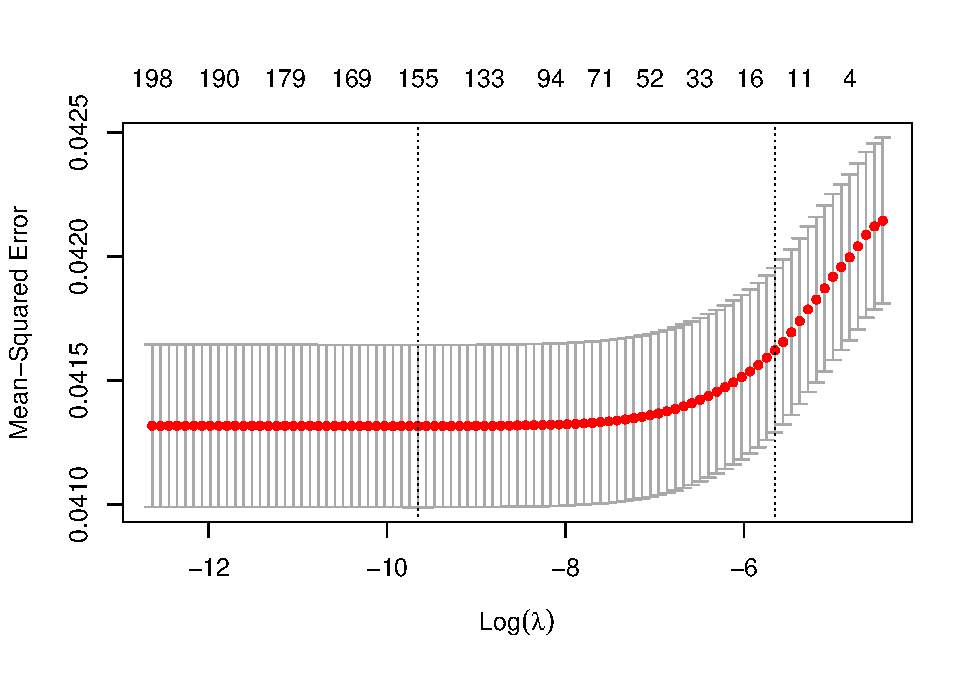
\includegraphics{dlassoMarkdown_files/figure-latex/unnamed-chunk-2-2.pdf}

\begin{Shaded}
\begin{Highlighting}[]
\CommentTok{# lasso}
\NormalTok{dlasso.}\FloatTok{2.1}\NormalTok{ <-}\StringTok{ }\KeywordTok{rlasso}\NormalTok{(formula2}\FloatTok{.1}\NormalTok{, }\DataTypeTok{data =}\NormalTok{ dat[train,], }
                     \DataTypeTok{lambda.start =}\NormalTok{ cv.lambda.}\FloatTok{2.1}\NormalTok{, }\DataTypeTok{post =}\NormalTok{ F)}
\CommentTok{#summary(dlasso.2.1, all = F)}
\NormalTok{focal1 <-}\StringTok{ }\KeywordTok{which}\NormalTok{(}\KeywordTok{coef}\NormalTok{(dlasso.}\FloatTok{2.1}\NormalTok{)[}\OperatorTok{-}\DecValTok{1}\NormalTok{]}\OperatorTok{!=}\DecValTok{0}\NormalTok{)}
\KeywordTok{length}\NormalTok{(focal1)}
\end{Highlighting}
\end{Shaded}

\begin{verbatim}
## [1] 74
\end{verbatim}

\begin{Shaded}
\begin{Highlighting}[]
\CommentTok{# travel time}
\NormalTok{formula2}\FloatTok{.2}\NormalTok{ <-}\StringTok{ }\KeywordTok{paste}\NormalTok{(}\KeywordTok{c}\NormalTok{(}\StringTok{"JWMNP"}\NormalTok{,varnames), }\DataTypeTok{collapse =} \StringTok{"~"}\NormalTok{)}
\CommentTok{# k-fold cv}
\NormalTok{xtrain <-}\StringTok{ }\KeywordTok{model.matrix}\NormalTok{(}\KeywordTok{as.formula}\NormalTok{(formula2}\FloatTok{.2}\NormalTok{), }\DataTypeTok{data =}\NormalTok{ dat[train,])[,}\OperatorTok{-}\DecValTok{1}\NormalTok{]}
\NormalTok{ytrain <-}\StringTok{ }\NormalTok{dat[train,]}\OperatorTok{$}\NormalTok{JWMNP}
\NormalTok{cv.lasso.}\FloatTok{2.2}\NormalTok{ <-}\StringTok{ }\KeywordTok{cv.glmnet}\NormalTok{(xtrain, ytrain, }\DataTypeTok{alpha =} \DecValTok{1}\NormalTok{)  }\CommentTok{# 1 for lasso}
\NormalTok{cv.lambda.}\FloatTok{2.2}\NormalTok{ <-}\StringTok{ }\NormalTok{cv.lasso.}\FloatTok{2.2}\OperatorTok{$}\NormalTok{lambda.min  }\CommentTok{# get smallest tuning parameter}
\NormalTok{cv.lambda.}\FloatTok{2.2}
\end{Highlighting}
\end{Shaded}

\begin{verbatim}
## [1] 0.0002590354
\end{verbatim}

\begin{Shaded}
\begin{Highlighting}[]
\KeywordTok{plot}\NormalTok{(cv.lasso.}\FloatTok{2.2}\NormalTok{)}
\end{Highlighting}
\end{Shaded}

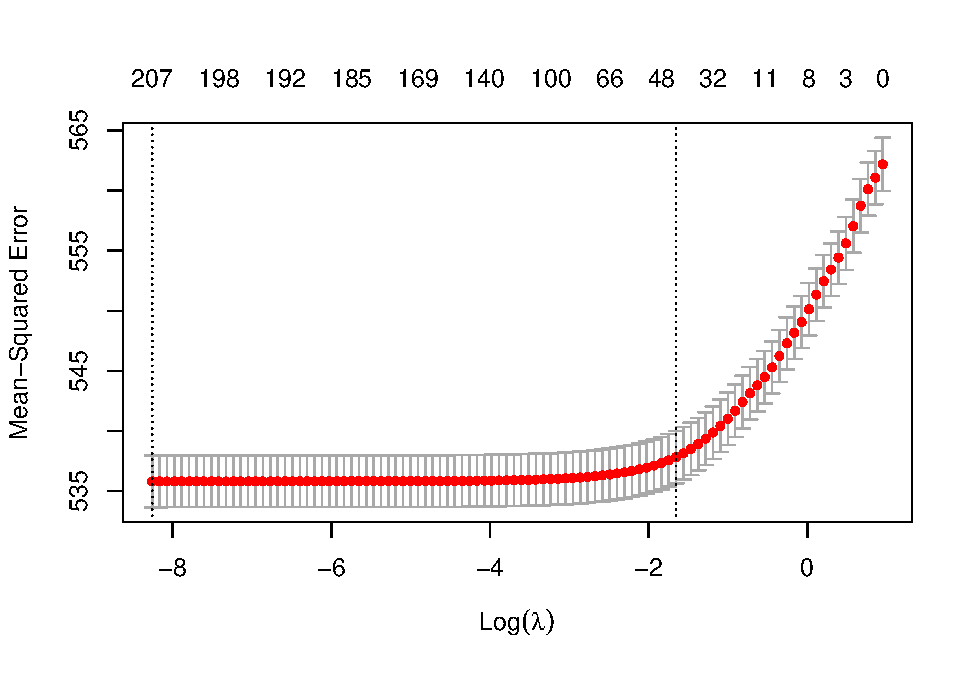
\includegraphics{dlassoMarkdown_files/figure-latex/unnamed-chunk-2-3.pdf}

\begin{Shaded}
\begin{Highlighting}[]
\CommentTok{# lasso}
\NormalTok{dlasso.}\FloatTok{2.2}\NormalTok{ <-}\StringTok{ }\KeywordTok{rlasso}\NormalTok{(formula2}\FloatTok{.2}\NormalTok{, }\DataTypeTok{data =}\NormalTok{ dat[train,], }
                     \DataTypeTok{lambda.start =}\NormalTok{ cv.lambda.}\FloatTok{2.2}\NormalTok{, }\DataTypeTok{post =}\NormalTok{ F)}
\CommentTok{#summary(dlasso.2.2, all = F)}
\NormalTok{focal2 <-}\StringTok{ }\KeywordTok{which}\NormalTok{(}\KeywordTok{coef}\NormalTok{(dlasso.}\FloatTok{2.2}\NormalTok{)[}\OperatorTok{-}\DecValTok{1}\NormalTok{]}\OperatorTok{!=}\DecValTok{0}\NormalTok{)}
\KeywordTok{length}\NormalTok{(focal2)}
\end{Highlighting}
\end{Shaded}

\begin{verbatim}
## [1] 81
\end{verbatim}

\begin{Shaded}
\begin{Highlighting}[]
\NormalTok{formula2}\FloatTok{.4}\NormalTok{ <-}\StringTok{ }\KeywordTok{paste}\NormalTok{(}\KeywordTok{c}\NormalTok{(}\StringTok{"JWTR"}\NormalTok{,varnames), }\DataTypeTok{collapse =} \StringTok{"~"}\NormalTok{)}
\CommentTok{# k-fold cv}
\NormalTok{xtrain <-}\StringTok{ }\KeywordTok{model.matrix}\NormalTok{(}\KeywordTok{as.formula}\NormalTok{(formula2}\FloatTok{.4}\NormalTok{), }\DataTypeTok{data =}\NormalTok{ dat[train,])[,}\OperatorTok{-}\DecValTok{1}\NormalTok{]}
\NormalTok{ytrain <-}\StringTok{ }\KeywordTok{drop.levels}\NormalTok{(dat[train,]}\OperatorTok{$}\NormalTok{JWTR) }\CommentTok{# factor level "11" has 0 observations}
\NormalTok{cv.lasso.}\FloatTok{2.4}\NormalTok{ <-}\StringTok{ }\KeywordTok{cv.glmnet}\NormalTok{(xtrain, ytrain, }\DataTypeTok{alpha =} \DecValTok{1}\NormalTok{, }\DataTypeTok{family =} \StringTok{"multinomial"}\NormalTok{, }\DataTypeTok{nfolds =} \DecValTok{3}\NormalTok{) }\CommentTok{# 1 for lasso}
\NormalTok{cv.lambda.}\FloatTok{2.4}\NormalTok{ <-}\StringTok{ }\NormalTok{cv.lasso.}\FloatTok{2.4}\OperatorTok{$}\NormalTok{lambda.min  }\CommentTok{# get smallest tuning parameter}
\NormalTok{cv.lambda.}\FloatTok{2.4}
\end{Highlighting}
\end{Shaded}

\begin{verbatim}
## [1] 3.31276e-05
\end{verbatim}

\begin{Shaded}
\begin{Highlighting}[]
\KeywordTok{plot}\NormalTok{(cv.lasso.}\FloatTok{2.4}\NormalTok{)}
\end{Highlighting}
\end{Shaded}

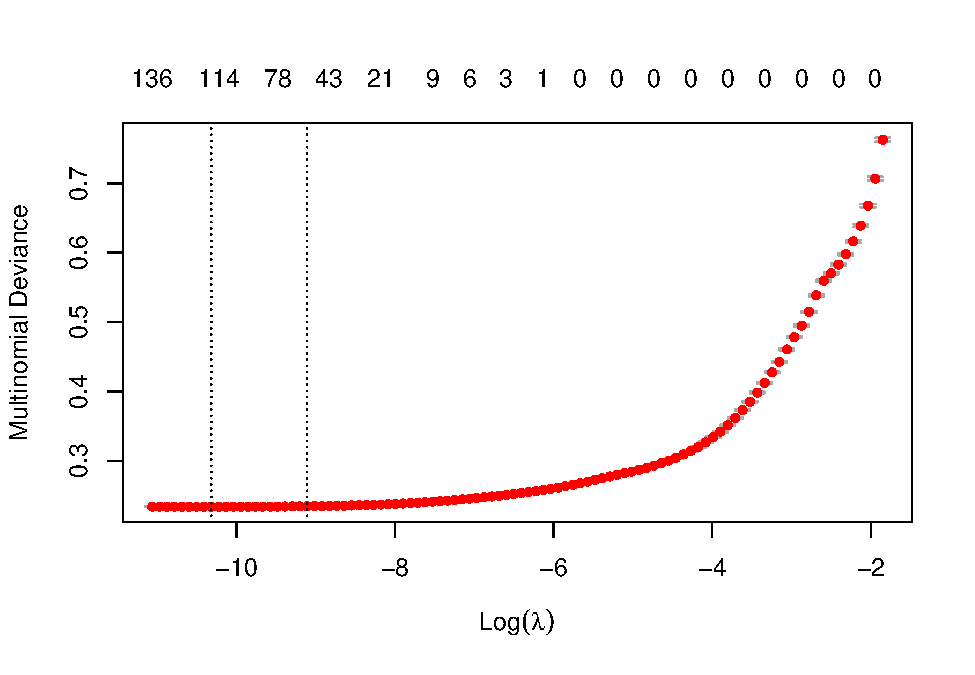
\includegraphics{dlassoMarkdown_files/figure-latex/unnamed-chunk-2-4.pdf}

\begin{Shaded}
\begin{Highlighting}[]
\CommentTok{# lasso}
\NormalTok{tempdat2 <-}\StringTok{ }\NormalTok{fastDummies}\OperatorTok{::}\KeywordTok{dummy_cols}\NormalTok{(dat)}
\NormalTok{focal4 <-}\StringTok{ }\KeywordTok{c}\NormalTok{()}
\ControlFlowTok{for}\NormalTok{ (ii }\ControlFlowTok{in} \DecValTok{1}\OperatorTok{:}\DecValTok{11}\NormalTok{) \{}
  \ControlFlowTok{if}\NormalTok{ (ii}\OperatorTok{<}\DecValTok{10}\NormalTok{) \{}
\NormalTok{    formula2.}\FloatTok{4.}\NormalTok{n <-}\StringTok{ }\KeywordTok{paste}\NormalTok{(}\KeywordTok{c}\NormalTok{(}\KeywordTok{paste}\NormalTok{(}\StringTok{"JWTR_0"}\NormalTok{,ii,}\DataTypeTok{sep=}\StringTok{""}\NormalTok{),varnames), }\DataTypeTok{collapse =} \StringTok{"~"}\NormalTok{)}
\NormalTok{    dlasso.}\DecValTok{2}\NormalTok{.}\FloatTok{4.}\NormalTok{n <-}\StringTok{ }\KeywordTok{rlasso}\NormalTok{(formula2.}\FloatTok{4.}\NormalTok{n, }\DataTypeTok{data =}\NormalTok{ tempdat2[train,], }
                           \DataTypeTok{lambda.start =}\NormalTok{ cv.lambda.}\FloatTok{2.4}\NormalTok{, }\DataTypeTok{post =}\NormalTok{ F)}
\NormalTok{    focal4.n <-}\StringTok{ }\KeywordTok{which}\NormalTok{(}\KeywordTok{coef}\NormalTok{(dlasso.}\DecValTok{2}\NormalTok{.}\FloatTok{4.}\NormalTok{n)[}\OperatorTok{-}\DecValTok{1}\NormalTok{]}\OperatorTok{!=}\DecValTok{0}\NormalTok{)}
\NormalTok{    focal4 <-}\StringTok{ }\KeywordTok{unique}\NormalTok{(}\KeywordTok{c}\NormalTok{(focal4, }\KeywordTok{names}\NormalTok{(focal4.n)))}
\NormalTok{  \} }\ControlFlowTok{else} \ControlFlowTok{if}\NormalTok{ (ii}\OperatorTok{==}\DecValTok{10}\NormalTok{) \{}
\NormalTok{    formula2.}\FloatTok{4.}\NormalTok{n <-}\StringTok{ }\KeywordTok{paste}\NormalTok{(}\KeywordTok{c}\NormalTok{(}\StringTok{"JWTR_10"}\NormalTok{,varnames), }\DataTypeTok{collapse =} \StringTok{"~"}\NormalTok{)}
\NormalTok{    dlasso.}\DecValTok{2}\NormalTok{.}\FloatTok{4.}\NormalTok{n <-}\StringTok{ }\KeywordTok{rlasso}\NormalTok{(formula2.}\FloatTok{4.}\NormalTok{n, }\DataTypeTok{data =}\NormalTok{ tempdat2[train,], }
                           \DataTypeTok{lambda.start =}\NormalTok{ cv.lambda.}\FloatTok{2.4}\NormalTok{, }\DataTypeTok{post =}\NormalTok{ F)}
\NormalTok{    focal4.n <-}\StringTok{ }\KeywordTok{which}\NormalTok{(}\KeywordTok{coef}\NormalTok{(dlasso.}\DecValTok{2}\NormalTok{.}\FloatTok{4.}\NormalTok{n)[}\OperatorTok{-}\DecValTok{1}\NormalTok{]}\OperatorTok{!=}\DecValTok{0}\NormalTok{)}
\NormalTok{    focal4 <-}\StringTok{ }\KeywordTok{unique}\NormalTok{(}\KeywordTok{c}\NormalTok{(focal4, }\KeywordTok{names}\NormalTok{(focal4.n)))}
\NormalTok{  \} }\ControlFlowTok{else} \ControlFlowTok{if}\NormalTok{ (ii}\OperatorTok{==}\DecValTok{11}\NormalTok{) \{}
\NormalTok{    formula2.}\FloatTok{4.}\NormalTok{n <-}\StringTok{ }\KeywordTok{paste}\NormalTok{(}\KeywordTok{c}\NormalTok{(}\StringTok{"JWTR_12"}\NormalTok{,varnames), }\DataTypeTok{collapse =} \StringTok{"~"}\NormalTok{)}
\NormalTok{    dlasso.}\DecValTok{2}\NormalTok{.}\FloatTok{4.}\NormalTok{n <-}\StringTok{ }\KeywordTok{rlasso}\NormalTok{(formula2.}\FloatTok{4.}\NormalTok{n, }\DataTypeTok{data =}\NormalTok{ tempdat2[train,], }
                           \DataTypeTok{lambda.start =}\NormalTok{ cv.lambda.}\FloatTok{2.4}\NormalTok{, }\DataTypeTok{post =}\NormalTok{ F)}
\NormalTok{    focal4.n <-}\StringTok{ }\KeywordTok{which}\NormalTok{(}\KeywordTok{coef}\NormalTok{(dlasso.}\DecValTok{2}\NormalTok{.}\FloatTok{4.}\NormalTok{n)[}\OperatorTok{-}\DecValTok{1}\NormalTok{]}\OperatorTok{!=}\DecValTok{0}\NormalTok{)}
\NormalTok{    focal4 <-}\StringTok{ }\KeywordTok{unique}\NormalTok{(}\KeywordTok{c}\NormalTok{(focal4, }\KeywordTok{names}\NormalTok{(focal4.n)))}
\NormalTok{  \}}
\NormalTok{\}}
\KeywordTok{length}\NormalTok{(focal4)}
\end{Highlighting}
\end{Shaded}

\begin{verbatim}
## [1] 213
\end{verbatim}

\begin{Shaded}
\begin{Highlighting}[]
\CommentTok{# STEP 3: Take union of all remainder potential variates}
\NormalTok{union <-}\StringTok{ }\KeywordTok{c}\NormalTok{(}\KeywordTok{names}\NormalTok{(control), }\KeywordTok{names}\NormalTok{(focal1), }\KeywordTok{names}\NormalTok{(focal2), focal4)}
\ControlFlowTok{if}\NormalTok{ (}\KeywordTok{any}\NormalTok{(}\KeywordTok{duplicated}\NormalTok{(union))}\OperatorTok{==}\NormalTok{T) \{}
\NormalTok{  union <-}\StringTok{ }\KeywordTok{unique}\NormalTok{(union)}
\NormalTok{\}}
\KeywordTok{length}\NormalTok{(union)}
\end{Highlighting}
\end{Shaded}

\begin{verbatim}
## [1] 219
\end{verbatim}

\begin{Shaded}
\begin{Highlighting}[]
\CommentTok{# STEP 4: do OLS of y on focals and kept potential variates}
\NormalTok{unionf <-}\StringTok{ }\KeywordTok{paste}\NormalTok{(}\KeywordTok{c}\NormalTok{(}\StringTok{"SameResidenceWorkplace*JWMNP+JWTR*JWMNP"}\NormalTok{,union), }\DataTypeTok{collapse =} \StringTok{"+"}\NormalTok{)}
\NormalTok{formula <-}\StringTok{ }\KeywordTok{paste}\NormalTok{(}\KeywordTok{c}\NormalTok{(}\StringTok{"log(IncomePovertyRatio)"}\NormalTok{, unionf), }\DataTypeTok{collapse =} \StringTok{"~"}\NormalTok{)}

\CommentTok{# name all extra variables created from doing LASSO}
\NormalTok{dattemp <-}\StringTok{ }\NormalTok{dat}
\ControlFlowTok{for}\NormalTok{ (i }\ControlFlowTok{in} \DecValTok{1}\OperatorTok{:}\DecValTok{500}\NormalTok{) \{ }\CommentTok{# look at formula and count how many new vars need to be made}
\NormalTok{  error <-}\StringTok{ }\KeywordTok{myTryCatch}\NormalTok{(olsDLasso1<-}\StringTok{ }\KeywordTok{lm}\NormalTok{(formula, }\DataTypeTok{data =}\NormalTok{ dattemp)) }\CommentTok{# }\AlertTok{CAUTION}
\NormalTok{  newvars <-}\StringTok{ }\KeywordTok{substr}\NormalTok{(error[[}\DecValTok{1}\NormalTok{]], }\DecValTok{45}\NormalTok{, }\KeywordTok{str_length}\NormalTok{(error[[}\DecValTok{1}\NormalTok{]])}\OperatorTok{-}\DecValTok{12}\NormalTok{)}
\NormalTok{  existingvars <-}\StringTok{ }\KeywordTok{names}\NormalTok{(dattemp)[}\KeywordTok{which}\NormalTok{(}\KeywordTok{str_detect}\NormalTok{(newvars, }\KeywordTok{names}\NormalTok{(dattemp)))]}
\NormalTok{  existingchars <-}\StringTok{ }\KeywordTok{sub}\NormalTok{(existingvars, }\StringTok{""}\NormalTok{, newvars)}
\NormalTok{  dattemp[,newvars] <-}\StringTok{ }\NormalTok{dattemp[,}\KeywordTok{which}\NormalTok{(}\KeywordTok{names}\NormalTok{(dattemp)}\OperatorTok{==}\NormalTok{existingvars)]}\OperatorTok{==}\NormalTok{existingchars}
\NormalTok{\}}
\end{Highlighting}
\end{Shaded}

\begin{verbatim}
## Warning in stri_length(string): argument is not an atomic vector; coercing

## Warning in stri_length(string): argument is not an atomic vector; coercing

## Warning in stri_length(string): argument is not an atomic vector; coercing

## Warning in stri_length(string): argument is not an atomic vector; coercing

## Warning in stri_length(string): argument is not an atomic vector; coercing

## Warning in stri_length(string): argument is not an atomic vector; coercing

## Warning in stri_length(string): argument is not an atomic vector; coercing

## Warning in stri_length(string): argument is not an atomic vector; coercing

## Warning in stri_length(string): argument is not an atomic vector; coercing

## Warning in stri_length(string): argument is not an atomic vector; coercing

## Warning in stri_length(string): argument is not an atomic vector; coercing

## Warning in stri_length(string): argument is not an atomic vector; coercing

## Warning in stri_length(string): argument is not an atomic vector; coercing

## Warning in stri_length(string): argument is not an atomic vector; coercing

## Warning in stri_length(string): argument is not an atomic vector; coercing

## Warning in stri_length(string): argument is not an atomic vector; coercing

## Warning in stri_length(string): argument is not an atomic vector; coercing

## Warning in stri_length(string): argument is not an atomic vector; coercing

## Warning in stri_length(string): argument is not an atomic vector; coercing

## Warning in stri_length(string): argument is not an atomic vector; coercing

## Warning in stri_length(string): argument is not an atomic vector; coercing

## Warning in stri_length(string): argument is not an atomic vector; coercing

## Warning in stri_length(string): argument is not an atomic vector; coercing

## Warning in stri_length(string): argument is not an atomic vector; coercing

## Warning in stri_length(string): argument is not an atomic vector; coercing

## Warning in stri_length(string): argument is not an atomic vector; coercing

## Warning in stri_length(string): argument is not an atomic vector; coercing

## Warning in stri_length(string): argument is not an atomic vector; coercing

## Warning in stri_length(string): argument is not an atomic vector; coercing

## Warning in stri_length(string): argument is not an atomic vector; coercing

## Warning in stri_length(string): argument is not an atomic vector; coercing

## Warning in stri_length(string): argument is not an atomic vector; coercing
\end{verbatim}

\begin{verbatim}
## Warning in sub(existingvars, "", newvars): argument 'pattern' has length > 1 and
## only the first element will be used
\end{verbatim}

\begin{verbatim}
## Warning in names(dattemp) == existingvars: longer object length is not a
## multiple of shorter object length
\end{verbatim}

\begin{verbatim}
## Warning in stri_length(string): argument is not an atomic vector; coercing
\end{verbatim}

\begin{verbatim}
## Warning in sub(existingvars, "", newvars): argument 'pattern' has length > 1 and
## only the first element will be used
\end{verbatim}

\begin{verbatim}
## Warning in stri_length(string): argument is not an atomic vector; coercing
\end{verbatim}

\begin{verbatim}
## Warning in sub(existingvars, "", newvars): argument 'pattern' has length > 1 and
## only the first element will be used
\end{verbatim}

\begin{verbatim}
## Warning in names(dattemp) == existingvars: longer object length is not a
## multiple of shorter object length
\end{verbatim}

\begin{verbatim}
## Warning in stri_length(string): argument is not an atomic vector; coercing
\end{verbatim}

\begin{verbatim}
## Warning in sub(existingvars, "", newvars): argument 'pattern' has length > 1 and
## only the first element will be used
\end{verbatim}

\begin{verbatim}
## Warning in stri_length(string): argument is not an atomic vector; coercing

## Warning in stri_length(string): argument is not an atomic vector; coercing

## Warning in stri_length(string): argument is not an atomic vector; coercing

## Warning in stri_length(string): argument is not an atomic vector; coercing

## Warning in stri_length(string): argument is not an atomic vector; coercing

## Warning in stri_length(string): argument is not an atomic vector; coercing

## Warning in stri_length(string): argument is not an atomic vector; coercing

## Warning in stri_length(string): argument is not an atomic vector; coercing

## Warning in stri_length(string): argument is not an atomic vector; coercing

## Warning in stri_length(string): argument is not an atomic vector; coercing

## Warning in stri_length(string): argument is not an atomic vector; coercing

## Warning in stri_length(string): argument is not an atomic vector; coercing

## Warning in stri_length(string): argument is not an atomic vector; coercing

## Warning in stri_length(string): argument is not an atomic vector; coercing

## Warning in stri_length(string): argument is not an atomic vector; coercing

## Warning in stri_length(string): argument is not an atomic vector; coercing

## Warning in stri_length(string): argument is not an atomic vector; coercing

## Warning in stri_length(string): argument is not an atomic vector; coercing

## Warning in stri_length(string): argument is not an atomic vector; coercing

## Warning in stri_length(string): argument is not an atomic vector; coercing

## Warning in stri_length(string): argument is not an atomic vector; coercing

## Warning in stri_length(string): argument is not an atomic vector; coercing

## Warning in stri_length(string): argument is not an atomic vector; coercing

## Warning in stri_length(string): argument is not an atomic vector; coercing

## Warning in stri_length(string): argument is not an atomic vector; coercing

## Warning in stri_length(string): argument is not an atomic vector; coercing

## Warning in stri_length(string): argument is not an atomic vector; coercing

## Warning in stri_length(string): argument is not an atomic vector; coercing

## Warning in stri_length(string): argument is not an atomic vector; coercing

## Warning in stri_length(string): argument is not an atomic vector; coercing

## Warning in stri_length(string): argument is not an atomic vector; coercing

## Warning in stri_length(string): argument is not an atomic vector; coercing

## Warning in stri_length(string): argument is not an atomic vector; coercing

## Warning in stri_length(string): argument is not an atomic vector; coercing

## Warning in stri_length(string): argument is not an atomic vector; coercing

## Warning in stri_length(string): argument is not an atomic vector; coercing

## Warning in stri_length(string): argument is not an atomic vector; coercing

## Warning in stri_length(string): argument is not an atomic vector; coercing

## Warning in stri_length(string): argument is not an atomic vector; coercing

## Warning in stri_length(string): argument is not an atomic vector; coercing

## Warning in stri_length(string): argument is not an atomic vector; coercing

## Warning in stri_length(string): argument is not an atomic vector; coercing

## Warning in stri_length(string): argument is not an atomic vector; coercing

## Warning in stri_length(string): argument is not an atomic vector; coercing

## Warning in stri_length(string): argument is not an atomic vector; coercing

## Warning in stri_length(string): argument is not an atomic vector; coercing

## Warning in stri_length(string): argument is not an atomic vector; coercing

## Warning in stri_length(string): argument is not an atomic vector; coercing

## Warning in stri_length(string): argument is not an atomic vector; coercing

## Warning in stri_length(string): argument is not an atomic vector; coercing

## Warning in stri_length(string): argument is not an atomic vector; coercing

## Warning in stri_length(string): argument is not an atomic vector; coercing

## Warning in stri_length(string): argument is not an atomic vector; coercing

## Warning in stri_length(string): argument is not an atomic vector; coercing

## Warning in stri_length(string): argument is not an atomic vector; coercing

## Warning in stri_length(string): argument is not an atomic vector; coercing

## Warning in stri_length(string): argument is not an atomic vector; coercing

## Warning in stri_length(string): argument is not an atomic vector; coercing

## Warning in stri_length(string): argument is not an atomic vector; coercing

## Warning in stri_length(string): argument is not an atomic vector; coercing

## Warning in stri_length(string): argument is not an atomic vector; coercing

## Warning in stri_length(string): argument is not an atomic vector; coercing

## Warning in stri_length(string): argument is not an atomic vector; coercing

## Warning in stri_length(string): argument is not an atomic vector; coercing

## Warning in stri_length(string): argument is not an atomic vector; coercing

## Warning in stri_length(string): argument is not an atomic vector; coercing

## Warning in stri_length(string): argument is not an atomic vector; coercing

## Warning in stri_length(string): argument is not an atomic vector; coercing

## Warning in stri_length(string): argument is not an atomic vector; coercing

## Warning in stri_length(string): argument is not an atomic vector; coercing

## Warning in stri_length(string): argument is not an atomic vector; coercing
\end{verbatim}

\begin{verbatim}
## Warning in sub(existingvars, "", newvars): argument 'pattern' has length > 1 and
## only the first element will be used
\end{verbatim}

\begin{verbatim}
## Warning in names(dattemp) == existingvars: longer object length is not a
## multiple of shorter object length
\end{verbatim}

\begin{verbatim}
## Warning in stri_length(string): argument is not an atomic vector; coercing
\end{verbatim}

\begin{verbatim}
## Warning in sub(existingvars, "", newvars): argument 'pattern' has length > 1 and
## only the first element will be used
\end{verbatim}

\begin{verbatim}
## Warning in stri_length(string): argument is not an atomic vector; coercing
\end{verbatim}

\begin{verbatim}
## Warning in sub(existingvars, "", newvars): argument 'pattern' has length > 1 and
## only the first element will be used
\end{verbatim}

\begin{verbatim}
## Warning in names(dattemp) == existingvars: longer object length is not a
## multiple of shorter object length
\end{verbatim}

\begin{verbatim}
## Warning in stri_length(string): argument is not an atomic vector; coercing

## Warning in stri_length(string): argument is not an atomic vector; coercing

## Warning in stri_length(string): argument is not an atomic vector; coercing

## Warning in stri_length(string): argument is not an atomic vector; coercing

## Warning in stri_length(string): argument is not an atomic vector; coercing

## Warning in stri_length(string): argument is not an atomic vector; coercing

## Warning in stri_length(string): argument is not an atomic vector; coercing

## Warning in stri_length(string): argument is not an atomic vector; coercing
\end{verbatim}

\begin{verbatim}
## Warning in sub(existingvars, "", newvars): argument 'pattern' has length > 1 and
## only the first element will be used
\end{verbatim}

\begin{verbatim}
## Warning in names(dattemp) == existingvars: longer object length is not a
## multiple of shorter object length
\end{verbatim}

\begin{verbatim}
## Warning in stri_length(string): argument is not an atomic vector; coercing

## Warning in stri_length(string): argument is not an atomic vector; coercing

## Warning in stri_length(string): argument is not an atomic vector; coercing

## Warning in stri_length(string): argument is not an atomic vector; coercing

## Warning in stri_length(string): argument is not an atomic vector; coercing

## Warning in stri_length(string): argument is not an atomic vector; coercing

## Warning in stri_length(string): argument is not an atomic vector; coercing

## Warning in stri_length(string): argument is not an atomic vector; coercing

## Warning in stri_length(string): argument is not an atomic vector; coercing

## Warning in stri_length(string): argument is not an atomic vector; coercing

## Warning in stri_length(string): argument is not an atomic vector; coercing

## Warning in stri_length(string): argument is not an atomic vector; coercing

## Warning in stri_length(string): argument is not an atomic vector; coercing

## Warning in stri_length(string): argument is not an atomic vector; coercing

## Warning in stri_length(string): argument is not an atomic vector; coercing

## Warning in stri_length(string): argument is not an atomic vector; coercing

## Warning in stri_length(string): argument is not an atomic vector; coercing

## Warning in stri_length(string): argument is not an atomic vector; coercing

## Warning in stri_length(string): argument is not an atomic vector; coercing

## Warning in stri_length(string): argument is not an atomic vector; coercing

## Warning in stri_length(string): argument is not an atomic vector; coercing

## Warning in stri_length(string): argument is not an atomic vector; coercing

## Warning in stri_length(string): argument is not an atomic vector; coercing

## Warning in stri_length(string): argument is not an atomic vector; coercing

## Warning in stri_length(string): argument is not an atomic vector; coercing
\end{verbatim}

\begin{verbatim}
## Warning in sub(existingvars, "", newvars): argument 'pattern' has length > 1 and
## only the first element will be used
\end{verbatim}

\begin{verbatim}
## Warning in stri_length(string): argument is not an atomic vector; coercing

## Warning in stri_length(string): argument is not an atomic vector; coercing

## Warning in stri_length(string): argument is not an atomic vector; coercing

## Warning in stri_length(string): argument is not an atomic vector; coercing
\end{verbatim}

\begin{verbatim}
## Warning in sub(existingvars, "", newvars): argument 'pattern' has length > 1 and
## only the first element will be used
\end{verbatim}

\begin{verbatim}
## Warning in stri_length(string): argument is not an atomic vector; coercing

## Warning in stri_length(string): argument is not an atomic vector; coercing

## Warning in stri_length(string): argument is not an atomic vector; coercing

## Warning in stri_length(string): argument is not an atomic vector; coercing
\end{verbatim}

\begin{verbatim}
## Error in sub(existingvars, "", newvars): invalid 'pattern' argument
\end{verbatim}

\begin{Shaded}
\begin{Highlighting}[]
\CommentTok{# start with declairing the new vars}
\KeywordTok{which}\NormalTok{(}\KeywordTok{colSums}\NormalTok{(}\KeywordTok{is.na}\NormalTok{(dattemp))}\OperatorTok{==}\KeywordTok{nrow}\NormalTok{(dattemp))}
\end{Highlighting}
\end{Shaded}

\begin{verbatim}
## SCIENGRLP1 SCIENGRLP2 
##        238        239
\end{verbatim}

\begin{Shaded}
\begin{Highlighting}[]
\NormalTok{dattemp}\OperatorTok{$}\NormalTok{SCIENGRLP1 <-}\StringTok{ }\NormalTok{dattemp}\OperatorTok{$}\NormalTok{SCIENGRLP }\OperatorTok{==}\StringTok{ "1"}
\NormalTok{dattemp}\OperatorTok{$}\NormalTok{SCIENGRLP2 <-}\StringTok{ }\NormalTok{dattemp}\OperatorTok{$}\NormalTok{SCIENGRLP }\OperatorTok{==}\StringTok{ "2"}

\KeywordTok{which}\NormalTok{(}\KeywordTok{lapply}\NormalTok{(dattemp, class)}\OperatorTok{==}\StringTok{"matrix"}\NormalTok{)}
\end{Highlighting}
\end{Shaded}

\begin{verbatim}
## MARHD2 MARHT2 MARHT3 MARHD8 
##    160    162    163    244
\end{verbatim}

\begin{Shaded}
\begin{Highlighting}[]
\NormalTok{dattemp}\OperatorTok{$}\NormalTok{MARHT3 <-}\StringTok{ }\NormalTok{dattemp}\OperatorTok{$}\NormalTok{MARHT }\OperatorTok{==}\StringTok{ "3"}
\NormalTok{dattemp}\OperatorTok{$}\NormalTok{MARHD2 <-}\StringTok{ }\NormalTok{dattemp}\OperatorTok{$}\NormalTok{MARHD }\OperatorTok{==}\StringTok{ "2"}
\NormalTok{dattemp}\OperatorTok{$}\NormalTok{MARHD8 <-}\StringTok{ }\NormalTok{dattemp}\OperatorTok{$}\NormalTok{MARHD }\OperatorTok{==}\StringTok{ "8"}
\NormalTok{dattemp}\OperatorTok{$}\NormalTok{MARHT2 <-}\StringTok{ }\NormalTok{dattemp}\OperatorTok{$}\NormalTok{MARHT }\OperatorTok{==}\StringTok{ "2"}

\CommentTok{# multicolinearity: get which variables have <2 unique values}
\NormalTok{multicol <-}\StringTok{ }\KeywordTok{names}\NormalTok{(}\KeywordTok{which}\NormalTok{(}\KeywordTok{sapply}\NormalTok{(dattemp[train,], }\ControlFlowTok{function}\NormalTok{(x) }\KeywordTok{length}\NormalTok{(}\KeywordTok{unique}\NormalTok{(x))}\OperatorTok{<}\DecValTok{2}\NormalTok{)))}
\CommentTok{# manually delete some of the rest (NA values in summary of lm, multicollinearity)}
\NormalTok{multicol <-}\StringTok{ }\KeywordTok{c}\NormalTok{(multicol,}
              \StringTok{"MSP3"}\NormalTok{,}\StringTok{"MSP4"}\NormalTok{,}\StringTok{"MSP5"}\NormalTok{,}\StringTok{"ENG1"}\NormalTok{,}\StringTok{"SCHL21"}\NormalTok{,}\StringTok{"DRIVESP6"}\NormalTok{,}
              \StringTok{"NATIVITY2"}\NormalTok{,}\StringTok{"SCHL18"}\NormalTok{,}\StringTok{"DECADE6"}\NormalTok{,}\StringTok{"WAOB4"}\NormalTok{)}
\NormalTok{union <-}\StringTok{ }\NormalTok{union[}\OperatorTok{-}\KeywordTok{which}\NormalTok{(union }\OperatorTok\StringTok{ }\NormalTok{multicol)] }\CommentTok{# delete them from formula}
\NormalTok{aliased <-}\StringTok{ }\KeywordTok{which}\NormalTok{(}\KeywordTok{summary}\NormalTok{(}\KeywordTok{lm}\NormalTok{(formula, }\DataTypeTok{data =}\NormalTok{ dattemp[train,]))}\OperatorTok{$}\NormalTok{aliased)}
\NormalTok{union <-}\StringTok{ }\NormalTok{union[}\OperatorTok{-}\KeywordTok{which}\NormalTok{(union }\OperatorTok\StringTok{ }\KeywordTok{names}\NormalTok{(aliased))]}

\CommentTok{# rewrite formula for OLS}
\NormalTok{unionf <-}\StringTok{ }\KeywordTok{paste}\NormalTok{(}\KeywordTok{c}\NormalTok{(}\StringTok{"SameResidenceWorkplace*JWMNP+JWTR*JWMNP"}\NormalTok{,union), }\DataTypeTok{collapse =} \StringTok{"+"}\NormalTok{)}
\NormalTok{formula <-}\StringTok{ }\KeywordTok{paste}\NormalTok{(}\KeywordTok{c}\NormalTok{(}\StringTok{"log(IncomePovertyRatio)"}\NormalTok{, unionf), }\DataTypeTok{collapse =} \StringTok{"~"}\NormalTok{)}

\CommentTok{# Training OLS regression post LASSO}
\NormalTok{olsDLasso1 <-}\StringTok{ }\KeywordTok{lm}\NormalTok{(formula, }\DataTypeTok{data =}\NormalTok{ dattemp[train,])}
\NormalTok{DMLresult <-}\StringTok{ }\KeywordTok{summary}\NormalTok{(olsDLasso1)}
\NormalTok{DMLresult}
\end{Highlighting}
\end{Shaded}

\begin{verbatim}
## 
## Call:
## lm(formula = formula, data = dattemp[train, ])
## 
## Residuals:
##     Min      1Q  Median      3Q     Max 
## -3.0233 -0.2576 -0.0282  0.2212  3.5316 
## 
## Coefficients:
##                                    Estimate Std. Error  t value Pr(>|t|)    
## (Intercept)                       1.918e+00  1.461e-01   13.124  < 2e-16 ***
## SameResidenceWorkplaceTRUE       -8.169e-02  4.054e-03  -20.149  < 2e-16 ***
## JWMNP                             1.431e-03  7.106e-05   20.141  < 2e-16 ***
## JWTR02                            1.093e-02  1.481e-02    0.737 0.460822    
## JWTR03                            3.399e-02  4.974e-02    0.683 0.494321    
## JWTR04                            2.488e-01  1.612e-02   15.434  < 2e-16 ***
## JWTR05                            3.626e-01  1.985e-02   18.263  < 2e-16 ***
## JWTR06                            3.288e-01  4.727e-02    6.955 3.53e-12 ***
## JWTR07                            8.782e-02  2.524e-02    3.479 0.000503 ***
## JWTR08                           -2.325e-02  2.305e-02   -1.009 0.313043    
## JWTR09                           -5.182e-02  1.791e-02   -2.894 0.003805 ** 
## JWTR10                           -6.349e-02  1.350e-02   -4.705 2.54e-06 ***
## JWTR12                            9.491e-03  1.469e-02    0.646 0.518130    
## SPORDER                          -6.923e-02  1.313e-03  -52.723  < 2e-16 ***
## PWGTP                             4.407e-05  6.578e-06    6.700 2.09e-11 ***
## AGEP                              4.456e-03  4.849e-04    9.191  < 2e-16 ***
## CIT3TRUE                         -3.097e-02  6.628e-03   -4.672 2.98e-06 ***
## CIT4TRUE                          9.808e-03  4.480e-03    2.189 0.028572 *  
## CIT5TRUE                         -1.488e-02  4.987e-03   -2.983 0.002857 ** 
## COW2TRUE                         -8.112e-02  1.805e-03  -44.949  < 2e-16 ***
## COW3TRUE                         -8.743e-02  1.869e-03  -46.793  < 2e-16 ***
## COW4TRUE                         -1.141e-01  2.277e-03  -50.089  < 2e-16 ***
## COW5TRUE                          6.980e-02  2.941e-03   23.732  < 2e-16 ***
## COW6TRUE                         -1.073e-01  2.194e-03  -48.883  < 2e-16 ***
## COW7TRUE                          9.960e-02  2.500e-03   39.844  < 2e-16 ***
## COW8TRUE                         -1.725e-01  1.103e-02  -15.645  < 2e-16 ***
## DDRS2TRUE                        -2.697e-02  8.954e-03   -3.012 0.002594 ** 
## DEYE2TRUE                         2.110e-02  5.392e-03    3.913 9.13e-05 ***
## DPHY2TRUE                         2.578e-02  5.036e-03    5.119 3.07e-07 ***
## DREM2TRUE                         3.432e-02  5.451e-03    6.296 3.06e-10 ***
## ENG2TRUE                         -9.786e-02  2.844e-03  -34.408  < 2e-16 ***
## ENG3TRUE                         -1.272e-01  3.656e-03  -34.784  < 2e-16 ***
## ENG4TRUE                         -1.138e-01  6.350e-03  -17.920  < 2e-16 ***
## FER1TRUE                          4.442e-02  5.013e-03    8.861  < 2e-16 ***
## FER2TRUE                          2.342e-02  2.036e-03   11.503  < 2e-16 ***
## GCL2TRUE                          2.570e-01  2.083e-02   12.342  < 2e-16 ***
## GCR2TRUE                          8.356e-02  4.472e-02    1.869 0.061677 .  
## HINS12TRUE                       -1.520e-01  1.500e-03 -101.372  < 2e-16 ***
## HINS22TRUE                       -1.308e-02  1.728e-03   -7.569 3.76e-14 ***
## HINS42TRUE                        9.252e-02  2.248e-03   41.164  < 2e-16 ***
## HINS52TRUE                       -2.228e-02  3.320e-03   -6.711 1.94e-11 ***
## HINS62TRUE                        5.436e-02  3.758e-03   14.465  < 2e-16 ***
## HINS72TRUE                        3.229e-03  8.499e-03    0.380 0.703987    
## LANX2TRUE                         1.159e-02  2.012e-03    5.758 8.50e-09 ***
## MAR2TRUE                         -2.623e-02  3.210e-03   -8.173 3.02e-16 ***
## MAR3TRUE                         -4.197e-02  1.670e-03  -25.131  < 2e-16 ***
## MAR4TRUE                         -4.869e-02  3.359e-03  -14.493  < 2e-16 ***
## MARHD2TRUE                       -2.075e-02  4.490e-03   -4.621 3.81e-06 ***
## MARHT2TRUE                       -5.534e-03  1.472e-03   -3.758 0.000171 ***
## MARHT3TRUE                       -2.639e-02  2.677e-03   -9.860  < 2e-16 ***
## MARHYP                           -3.978e-04  6.967e-05   -5.710 1.13e-08 ***
## MIG2TRUE                         -5.720e-02  8.815e-03   -6.489 8.64e-11 ***
## MIG3TRUE                         -1.420e-02  1.707e-03   -8.323  < 2e-16 ***
## NWAB2TRUE                        -2.978e-02  9.740e-03   -3.057 0.002234 ** 
## NWAV5TRUE                         7.657e-03  5.268e-03    1.454 0.146062    
## NWLA3TRUE                         3.213e-03  1.069e-02    0.301 0.763636    
## NWLK3TRUE                         8.442e-02  7.974e-03   10.586  < 2e-16 ***
## NWRE2TRUE                         6.009e-02  1.167e-02    5.149 2.62e-07 ***
## RELP01TRUE                       -1.579e-01  1.740e-03  -90.721  < 2e-16 ***
## RELP02TRUE                       -2.422e-01  4.139e-03  -58.517  < 2e-16 ***
## RELP03TRUE                       -2.222e-01  2.175e-02  -10.218  < 2e-16 ***
## RELP04TRUE                       -2.501e-01  1.523e-02  -16.422  < 2e-16 ***
## RELP05TRUE                       -2.344e-01  7.721e-03  -30.357  < 2e-16 ***
## RELP06TRUE                       -2.428e-01  7.102e-03  -34.192  < 2e-16 ***
## RELP07TRUE                       -2.017e-01  1.581e-02  -12.757  < 2e-16 ***
## RELP08TRUE                       -3.037e-01  1.467e-02  -20.705  < 2e-16 ***
## RELP09TRUE                       -2.874e-01  7.891e-03  -36.425  < 2e-16 ***
## RELP10TRUE                       -2.442e-01  8.130e-03  -30.035  < 2e-16 ***
## RELP11TRUE                       -2.412e-01  1.051e-02  -22.950  < 2e-16 ***
## RELP12TRUE                       -2.277e-01  7.150e-03  -31.849  < 2e-16 ***
## RELP13TRUE                       -2.062e-01  4.674e-03  -44.118  < 2e-16 ***
## RELP15TRUE                       -2.442e-01  7.903e-03  -30.895  < 2e-16 ***
## RELP17TRUE                       -2.786e-01  1.332e-02  -20.911  < 2e-16 ***
## SCHL04TRUE                       -1.043e-01  3.053e-02   -3.416 0.000635 ***
## SCHL05TRUE                       -1.342e-01  2.178e-02   -6.160 7.27e-10 ***
## SCHL06TRUE                       -1.007e-01  1.467e-02   -6.863 6.73e-12 ***
## SCHL07TRUE                       -1.055e-01  1.708e-02   -6.175 6.61e-10 ***
## SCHL08TRUE                       -1.064e-01  1.370e-02   -7.771 7.82e-15 ***
## SCHL09TRUE                       -1.012e-01  6.870e-03  -14.725  < 2e-16 ***
## SCHL10TRUE                       -1.151e-01  1.224e-02   -9.400  < 2e-16 ***
## SCHL11TRUE                       -8.077e-02  7.093e-03  -11.386  < 2e-16 ***
## SCHL12TRUE                       -1.061e-01  5.992e-03  -17.709  < 2e-16 ***
## SCHL13TRUE                       -1.301e-01  5.561e-03  -23.397  < 2e-16 ***
## SCHL14TRUE                       -1.185e-01  5.176e-03  -22.892  < 2e-16 ***
## SCHL15TRUE                       -9.016e-02  4.420e-03  -20.397  < 2e-16 ***
## SCHL16TRUE                       -6.246e-02  2.171e-03  -28.772  < 2e-16 ***
## SCHL17TRUE                       -8.702e-02  3.278e-03  -26.545  < 2e-16 ***
## SCHL19TRUE                        3.397e-02  2.304e-03   14.741  < 2e-16 ***
## SCHL20TRUE                        6.445e-02  2.424e-03   26.591  < 2e-16 ***
## SCHL22TRUE                        1.233e-01  2.478e-03   49.751  < 2e-16 ***
## SCHL23TRUE                        3.437e-01  8.596e-03   39.985  < 2e-16 ***
## SCHL24TRUE                        2.175e-01  6.802e-03   31.977  < 2e-16 ***
## SEX2TRUE                         -7.976e-02  2.289e-02   -3.484 0.000493 ***
## WKHP                              1.365e-02  4.765e-05  286.546  < 2e-16 ***
## WKW2TRUE                         -7.342e-02  3.505e-03  -20.948  < 2e-16 ***
## WKW3TRUE                         -1.582e-01  2.339e-03  -67.629  < 2e-16 ***
## WKW4TRUE                         -2.789e-01  2.820e-03  -98.897  < 2e-16 ***
## WKW5TRUE                         -4.105e-01  3.867e-03 -106.155  < 2e-16 ***
## WKW6TRUE                         -5.210e-01  3.940e-03 -132.240  < 2e-16 ***
## DECADE3TRUE                       3.593e-02  6.193e-03    5.801 6.58e-09 ***
## DECADE4TRUE                       2.350e-02  4.386e-03    5.359 8.37e-08 ***
## DECADE7TRUE                      -2.040e-02  3.331e-03   -6.125 9.10e-10 ***
## DECADE8TRUE                      -5.498e-02  4.133e-03  -13.302  < 2e-16 ***
## DIS2TRUE                          4.190e-02  4.841e-03    8.655  < 2e-16 ***
## DRIVESP1TRUE                     -1.330e-02  1.269e-02   -1.049 0.294402    
## DRIVESP2TRUE                     -6.237e-02  1.281e-02   -4.870 1.12e-06 ***
## DRIVESP3TRUE                     -5.937e-02  1.334e-02   -4.451 8.55e-06 ***
## DRIVESP4TRUE                     -5.789e-02  1.438e-02   -4.025 5.70e-05 ***
## DRIVESP5TRUE                     -3.096e-02  1.578e-02   -1.962 0.049801 *  
## MSP2TRUE                         -1.459e-02  3.143e-03   -4.642 3.45e-06 ***
## PAOC1TRUE                        -9.965e-02  2.304e-02   -4.324 1.53e-05 ***
## PAOC2TRUE                        -1.329e-01  2.291e-02   -5.803 6.53e-09 ***
## PAOC4TRUE                        -1.321e-01  2.288e-02   -5.773 7.80e-09 ***
## QTRBIR3TRUE                       3.229e-03  1.189e-03    2.715 0.006626 ** 
## RACAIAN1TRUE                     -2.852e-02  5.081e-03   -5.612 2.00e-08 ***
## RACASN1TRUE                       6.301e-02  4.437e-03   14.203  < 2e-16 ***
## RACBLK1TRUE                      -6.564e-02  4.108e-03  -15.980  < 2e-16 ***
## RACPI1TRUE                       -2.557e-02  1.224e-02   -2.088 0.036787 *  
## RACWHT1TRUE                       2.257e-02  3.879e-03    5.817 6.00e-09 ***
## SCIENGRLP1TRUE                    3.276e-01  3.554e-03   92.186  < 2e-16 ***
## SCIENGRLP2TRUE                    2.506e-01  2.330e-03  107.536  < 2e-16 ***
## WAOB2TRUE                         1.641e-02  5.217e-02    0.315 0.753068    
## WAOB3TRUE                        -1.879e-02  4.167e-03   -4.508 6.54e-06 ***
## WAOB5TRUE                         6.072e-02  4.846e-03   12.528  < 2e-16 ***
## WAOB6TRUE                        -2.510e-02  6.657e-03   -3.771 0.000163 ***
## WAOB7TRUE                         1.233e-01  8.684e-03   14.196  < 2e-16 ***
## WAOB8TRUE                         1.105e-01  1.535e-02    7.198 6.13e-13 ***
## AGEP_HINS31                       1.562e-03  2.448e-04    6.382 1.75e-10 ***
## SCIENGP_SCHL01                   -9.545e-02  5.379e-03  -17.745  < 2e-16 ***
## SCIENGP1_SCHL22                   1.123e-01  3.115e-03   36.039  < 2e-16 ***
## SCIENGP1_SCHL23                   2.355e-01  5.968e-03   39.456  < 2e-16 ***
## SCIENGP1_SCHL24                   1.742e-01  7.863e-03   22.154  < 2e-16 ***
## SCIENGRLP1_SCHL22                 7.894e-03  5.833e-03    1.353 0.175985    
## SCIENGRLP2_SCHL23                 1.390e-02  9.687e-03    1.435 0.151276    
## SCIENGRLP1_SCHL24                 7.851e-02  1.269e-02    6.188 6.08e-10 ***
## AGEP_VETERAN                      5.122e-04  1.336e-04    3.834 0.000126 ***
## AGEP_GCL                          6.289e-03  9.141e-04    6.880 5.99e-12 ***
## DOUT2TRUE                        -7.836e-03  6.693e-03   -1.171 0.241662    
## MARHD8TRUE                       -5.994e-03  1.348e-02   -0.445 0.656588    
## NWAB3TRUE                         8.029e-04  1.048e-02    0.077 0.938949    
## RACNH1TRUE                       -1.854e-03  1.226e-02   -0.151 0.879789    
## RACSOR1TRUE                       8.821e-03  4.479e-03    1.969 0.048897 *  
## AGEP_GCL2                         6.915e-04  4.779e-04    1.447 0.147896    
## CIT2TRUE                         -4.371e-02  5.260e-02   -0.831 0.406013    
## DEAR2TRUE                         1.772e-03  5.003e-03    0.354 0.723115    
## GCL1TRUE                          1.786e-01  4.101e-02    4.355 1.33e-05 ***
## NWLA2TRUE                        -1.020e-02  1.103e-02   -0.925 0.354919    
## DECADE5TRUE                       1.040e-03  3.506e-03    0.297 0.766786    
## SCIENGP1_SCHL21                   7.754e-02  2.292e-03   33.827  < 2e-16 ***
## VETERAN                          -1.758e-02  7.315e-03   -2.404 0.016228 *  
## GCM1TRUE                          1.106e-02  1.711e-02    0.646 0.518256    
## GCM2TRUE                         -6.377e-03  1.695e-02   -0.376 0.706680    
## GCM4TRUE                          2.230e-02  1.348e-02    1.654 0.098059 .  
## HINS32TRUE                        4.964e-02  1.664e-02    2.983 0.002857 ** 
## NWAV3TRUE                        -2.263e-02  8.308e-03   -2.723 0.006466 ** 
## SCHL02TRUE                       -3.983e-02  3.363e-02   -1.184 0.236227    
## SCHL03TRUE                       -6.848e-02  3.793e-02   -1.805 0.071006 .  
## DECADE1TRUE                       1.600e-02  3.138e-02    0.510 0.610265    
## DECADE2TRUE                       5.866e-03  1.042e-02    0.563 0.573573    
## PAOC3TRUE                        -1.105e-01  2.305e-02   -4.795 1.63e-06 ***
## AGEP_GCR1                         1.164e-03  7.613e-04    1.529 0.126288    
## GCM3TRUE                          2.665e-03  1.223e-02    0.218 0.827452    
## NWAV2TRUE                        -8.294e-03  1.418e-02   -0.585 0.558620    
## NWLK2TRUE                         7.811e-02  7.118e-03   10.973  < 2e-16 ***
## NWRE3TRUE                         3.179e-02  1.178e-02    2.698 0.006973 ** 
## QTRBIR2TRUE                       2.164e-03  1.219e-03    1.776 0.075757 .  
## SameResidenceWorkplaceTRUE:JWMNP  4.053e-06  7.287e-05    0.056 0.955644    
## JWMNP:JWTR02                     -4.712e-04  1.278e-04   -3.688 0.000226 ***
## JWMNP:JWTR03                     -4.075e-04  1.036e-03   -0.393 0.693954    
## JWMNP:JWTR04                     -3.007e-03  1.743e-04  -17.252  < 2e-16 ***
## JWMNP:JWTR05                     -1.646e-03  1.913e-04   -8.605  < 2e-16 ***
## JWMNP:JWTR06                     -1.650e-03  6.101e-04   -2.704 0.006852 ** 
## JWMNP:JWTR07                     -1.013e-03  7.045e-04   -1.439 0.150256    
## JWMNP:JWTR08                      3.503e-04  6.298e-04    0.556 0.578017    
## JWMNP:JWTR09                      1.478e-03  4.447e-04    3.325 0.000885 ***
## JWMNP:JWTR10                      4.182e-04  2.490e-04    1.680 0.093044 .  
## JWMNP:JWTR12                     -4.323e-05  1.213e-04   -0.356 0.721470    
## ---
## Signif. codes:  0 '***' 0.001 '**' 0.01 '*' 0.05 '.' 0.1 ' ' 1
## 
## Residual standard error: 0.435 on 781192 degrees of freedom
## Multiple R-squared:  0.5123, Adjusted R-squared:  0.5122 
## F-statistic:  4662 on 176 and 781192 DF,  p-value: < 2.2e-16
\end{verbatim}

\begin{Shaded}
\begin{Highlighting}[]
\CommentTok{# Test Prediction}
\NormalTok{pred.olsDLasso}\FloatTok{.1}\NormalTok{ <-}\StringTok{ }\KeywordTok{predict}\NormalTok{(olsDLasso1, }\DataTypeTok{newdata =}\NormalTok{ dattemp[}\OperatorTok{-}\NormalTok{train,])}
\KeywordTok{summary}\NormalTok{(pred.olsDLasso}\FloatTok{.1}\NormalTok{)}
\end{Highlighting}
\end{Shaded}

\begin{verbatim}
##    Min. 1st Qu.  Median    Mean 3rd Qu.    Max. 
## -0.3127  1.9878  2.2644  2.2562  2.5408  4.2571
\end{verbatim}

\begin{Shaded}
\begin{Highlighting}[]
\KeywordTok{length}\NormalTok{(}\KeywordTok{na.omit}\NormalTok{(pred.olsDLasso}\FloatTok{.1}\NormalTok{)) }\CommentTok{# count remaining observations}
\end{Highlighting}
\end{Shaded}

\begin{verbatim}
## [1] 195343
\end{verbatim}

\begin{Shaded}
\begin{Highlighting}[]
\CommentTok{# test error}
\NormalTok{mse}\FloatTok{.1}\NormalTok{ <-}\StringTok{ }\KeywordTok{mean}\NormalTok{((pred.olsDLasso}\FloatTok{.1}\OperatorTok{-}\KeywordTok{log}\NormalTok{(dattemp[}\OperatorTok{-}\NormalTok{train,]}\OperatorTok{$}\NormalTok{IncomePovertyRatio))}\OperatorTok{^}\DecValTok{2}\NormalTok{, }\DataTypeTok{na.rm=}\NormalTok{T)}
\NormalTok{mse}\FloatTok{.1}
\end{Highlighting}
\end{Shaded}

\begin{verbatim}
## [1] 0.1894029
\end{verbatim}

\hypertarget{result-1-analysis-hypothesis-testing}{%
\subsection{Result 1 Analysis \& Hypothesis
Testing}\label{result-1-analysis-hypothesis-testing}}

\begin{Shaded}
\begin{Highlighting}[]
\CommentTok{# 3 Ways of getting Test R2}
\NormalTok{y <-}\StringTok{ }\KeywordTok{log}\NormalTok{(dattemp[}\OperatorTok{-}\NormalTok{train,]}\OperatorTok{$}\NormalTok{IncomePovertyRatio)}\OperatorTok{-}\KeywordTok{mean}\NormalTok{(}\KeywordTok{log}\NormalTok{(dattemp[}\OperatorTok{-}\NormalTok{train,]}\OperatorTok{$}\NormalTok{IncomePovertyRatio))}
\NormalTok{yhat <-}\StringTok{ }\NormalTok{pred.olsDLasso}\FloatTok{.1}\OperatorTok{-}\KeywordTok{mean}\NormalTok{(pred.olsDLasso}\FloatTok{.1}\NormalTok{)}
\NormalTok{u <-}\StringTok{ }\NormalTok{y }\OperatorTok{-}\StringTok{ }\NormalTok{yhat}
\CommentTok{# 1:}
\CommentTok{# R2 = yhat*yhat/yTy}
\NormalTok{r2_}\DecValTok{1}\NormalTok{ <-}\StringTok{ }\NormalTok{(yhat }\OperatorTok\StringTok{ }\NormalTok{yhat)}\OperatorTok{/}\NormalTok{(y }\OperatorTok\StringTok{ }\NormalTok{y)}
\NormalTok{r2_}\DecValTok{1}
\end{Highlighting}
\end{Shaded}

\begin{verbatim}
##           [,1]
## [1,] 0.5125579
\end{verbatim}

\begin{Shaded}
\begin{Highlighting}[]
\CommentTok{# 2:}
\CommentTok{# R2 = 1- SSR/SST = 1- uTu/yTy}
\NormalTok{r2_}\DecValTok{2}\NormalTok{ <-}\StringTok{ }\DecValTok{1} \OperatorTok{-}\StringTok{ }\NormalTok{(u }\OperatorTok\StringTok{ }\NormalTok{u)}\OperatorTok{/}\NormalTok{(y }\OperatorTok\StringTok{ }\NormalTok{y)}
\NormalTok{r2_}\DecValTok{2}
\end{Highlighting}
\end{Shaded}

\begin{verbatim}
##           [,1]
## [1,] 0.5089613
\end{verbatim}

\begin{Shaded}
\begin{Highlighting}[]
\CommentTok{# 3:}
\CommentTok{# R2 = corr(y, yhat)^2, "fair r-squared"}
\NormalTok{r2_}\DecValTok{3}\NormalTok{ <-}\StringTok{ }\KeywordTok{cor.test}\NormalTok{(y, yhat, }\DataTypeTok{use =} \StringTok{"complete.obs"}\NormalTok{)}
\CommentTok{# now, square the correlation coefficient}
\NormalTok{r2_}\DecValTok{3}
\end{Highlighting}
\end{Shaded}

\begin{verbatim}
## 
##  Pearson's product-moment correlation
## 
## data:  y and yhat
## t = 449.97, df = 195341, p-value < 2.2e-16
## alternative hypothesis: true correlation is not equal to 0
## 95 percent confidence interval:
##  0.7112352 0.7155903
## sample estimates:
##       cor 
## 0.7134197
\end{verbatim}

\begin{Shaded}
\begin{Highlighting}[]
\NormalTok{r2_}\DecValTok{3}\OperatorTok{$}\NormalTok{estimate}\OperatorTok{^}\DecValTok{2}
\end{Highlighting}
\end{Shaded}

\begin{verbatim}
##       cor 
## 0.5089676
\end{verbatim}

\begin{Shaded}
\begin{Highlighting}[]
\CommentTok{# False Discovery Rate control}
\NormalTok{p <-}\StringTok{ }\KeywordTok{as.data.frame}\NormalTok{(DMLresult}\OperatorTok{$}\NormalTok{coefficients[,}\DecValTok{4}\NormalTok{])}
\NormalTok{sigcode <-}\StringTok{ }\KeywordTok{cut}\NormalTok{(p[,}\DecValTok{1}\NormalTok{], }\DataTypeTok{breaks =} \KeywordTok{c}\NormalTok{(}\OperatorTok{-}\OtherTok{Inf}\NormalTok{, }\FloatTok{0.001}\NormalTok{, }\FloatTok{0.01}\NormalTok{, }\FloatTok{0.05}\NormalTok{, }\FloatTok{0.1}\NormalTok{, }\DecValTok{1}\NormalTok{), }
               \DataTypeTok{labels =} \KeywordTok{c}\NormalTok{(}\StringTok{"***"}\NormalTok{, }\StringTok{"**"}\NormalTok{, }\StringTok{"*"}\NormalTok{, }\StringTok{"."}\NormalTok{, }\StringTok{" "}\NormalTok{))}
\NormalTok{p}\OperatorTok{$}\StringTok{""}\NormalTok{ <-}\StringTok{ }\NormalTok{sigcode}

\CommentTok{# sort by increasing p-value}
\NormalTok{p <-}\StringTok{ }\NormalTok{p[}\KeywordTok{order}\NormalTok{(p}\OperatorTok{$}\StringTok{`}\DataTypeTok{DMLresult$coefficients[, 4]}\StringTok{`}\NormalTok{),]}
\NormalTok{p}\OperatorTok{$}\NormalTok{BY <-}\StringTok{ }\DecValTok{0}
\NormalTok{m <-}\StringTok{ }\KeywordTok{nrow}\NormalTok{(p)}
\NormalTok{Q =}\StringTok{ }\FloatTok{0.10}  \CommentTok{# 10%}
\NormalTok{cm=}\DecValTok{0}
\ControlFlowTok{for}\NormalTok{ (ii }\ControlFlowTok{in} \DecValTok{1}\OperatorTok{:}\NormalTok{m) \{}
\NormalTok{  cm =}\StringTok{ }\NormalTok{cm }\OperatorTok{+}\StringTok{ }\DecValTok{1}\OperatorTok{/}\NormalTok{ii}
\NormalTok{  p[ii,}\DecValTok{3}\NormalTok{] <-}\StringTok{ }\NormalTok{ii}\OperatorTok{/}\NormalTok{m}\OperatorTok{/}\NormalTok{cm}\OperatorTok{*}\NormalTok{Q}
\NormalTok{\}}
\NormalTok{noreject <-}\StringTok{ }\NormalTok{(}\OperatorTok{!}\NormalTok{(p[,}\DecValTok{1}\NormalTok{] }\OperatorTok{<}\StringTok{ }\NormalTok{p[,}\DecValTok{3}\NormalTok{]))}
\KeywordTok{plot}\NormalTok{(p}\OperatorTok{$}\StringTok{`}\DataTypeTok{DMLresult$coefficients[, 4]}\StringTok{`}\NormalTok{,}\DataTypeTok{ylab=}\StringTok{"P-Value"}\NormalTok{, }\DataTypeTok{col =} \KeywordTok{ifelse}\NormalTok{(noreject,}\StringTok{'red'}\NormalTok{,}\StringTok{'black'}\NormalTok{))}
\end{Highlighting}
\end{Shaded}

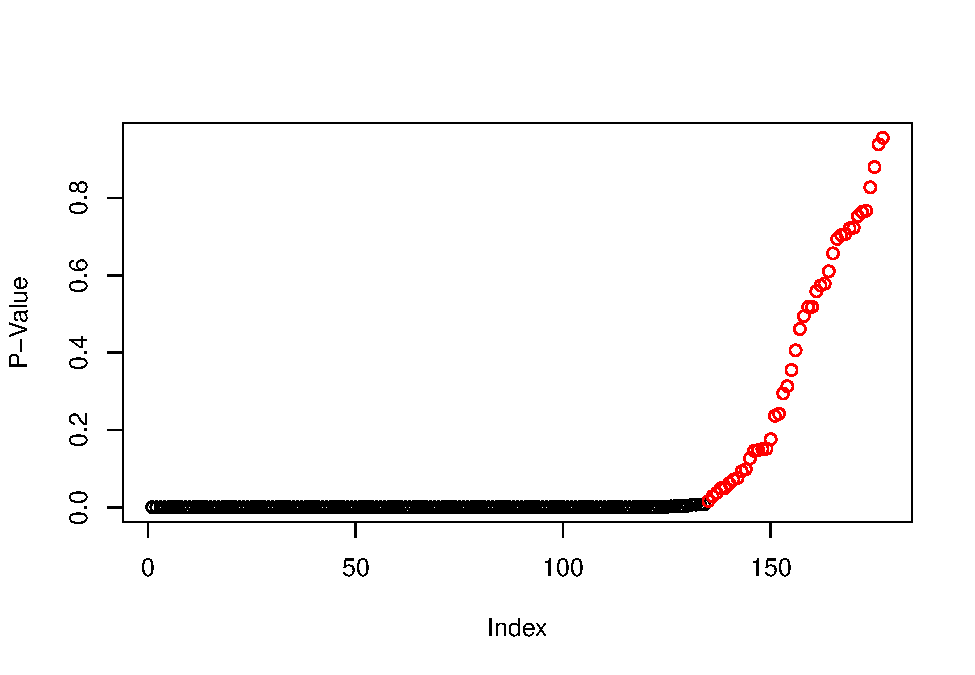
\includegraphics{dlassoMarkdown_files/figure-latex/unnamed-chunk-3-1.pdf}

\begin{Shaded}
\begin{Highlighting}[]
\NormalTok{noreject <-}\StringTok{ }\KeywordTok{which}\NormalTok{(noreject)}
\NormalTok{p <-}\StringTok{ }\NormalTok{p[noreject,]   }\CommentTok{# these one's we cannot reject the null}
\KeywordTok{names}\NormalTok{(p) <-}\StringTok{ }\KeywordTok{c}\NormalTok{(}\StringTok{"p-value"}\NormalTok{,}\StringTok{"Sig. Level"}\NormalTok{,}\StringTok{"BY Stat"}\NormalTok{)}
\NormalTok{p}
\end{Highlighting}
\end{Shaded}

\begin{verbatim}
##                                     p-value Sig. Level    BY Stat
## VETERAN                          0.01622773          * 0.01390240
## CIT4TRUE                         0.02857226          * 0.01398663
## RACPI1TRUE                       0.03678683          * 0.01407078
## RACSOR1TRUE                      0.04889671          * 0.01415484
## DRIVESP5TRUE                     0.04980121          * 0.01423881
## GCR2TRUE                         0.06167725          . 0.01432270
## SCHL03TRUE                       0.07100579          . 0.01440650
## QTRBIR2TRUE                      0.07575731          . 0.01449022
## JWMNP:JWTR10                     0.09304410          . 0.01457386
## GCM4TRUE                         0.09805948          . 0.01465741
## AGEP_GCR1                        0.12628818            0.01474089
## NWAV5TRUE                        0.14606246            0.01482428
## AGEP_GCL2                        0.14789649            0.01490759
## JWMNP:JWTR07                     0.15025585            0.01499082
## SCIENGRLP2_SCHL23                0.15127602            0.01507397
## SCIENGRLP1_SCHL22                0.17598520            0.01515704
## SCHL02TRUE                       0.23622737            0.01524004
## DOUT2TRUE                        0.24166238            0.01532296
## DRIVESP1TRUE                     0.29440172            0.01540580
## JWTR08                           0.31304290            0.01548857
## NWLA2TRUE                        0.35491891            0.01557126
## CIT2TRUE                         0.40601337            0.01565387
## JWTR02                           0.46082218            0.01573642
## JWTR03                           0.49432147            0.01581889
## JWTR12                           0.51813036            0.01590128
## GCM1TRUE                         0.51825607            0.01598361
## NWAV2TRUE                        0.55862008            0.01606586
## DECADE2TRUE                      0.57357341            0.01614804
## JWMNP:JWTR08                     0.57801715            0.01623016
## DECADE1TRUE                      0.61026469            0.01631220
## MARHD8TRUE                       0.65658784            0.01639417
## JWMNP:JWTR03                     0.69395359            0.01647607
## HINS72TRUE                       0.70398697            0.01655791
## GCM2TRUE                         0.70667974            0.01663968
## JWMNP:JWTR12                     0.72146983            0.01672138
## DEAR2TRUE                        0.72311468            0.01680301
## WAOB2TRUE                        0.75306776            0.01688458
## NWLA3TRUE                        0.76363569            0.01696608
## DECADE5TRUE                      0.76678592            0.01704751
## GCM3TRUE                         0.82745213            0.01712888
## RACNH1TRUE                       0.87978946            0.01721019
## NWAB3TRUE                        0.93894933            0.01729143
## SameResidenceWorkplaceTRUE:JWMNP 0.95564425            0.01737261
\end{verbatim}

\begin{Shaded}
\begin{Highlighting}[]
\CommentTok{# get BY-adjusted p-values}
\NormalTok{pBY <-}\StringTok{ }\KeywordTok{as.data.frame}\NormalTok{(}\KeywordTok{p.adjust}\NormalTok{(p[,}\DecValTok{1}\NormalTok{], }\DataTypeTok{method =} \StringTok{"BY"}\NormalTok{))   }\CommentTok{#Benjamini-Yekutieli}
\KeywordTok{rownames}\NormalTok{(pBY) <-}\StringTok{ }\KeywordTok{rownames}\NormalTok{(p)}
\NormalTok{adjsigcode <-}\StringTok{ }\KeywordTok{cut}\NormalTok{(pBY[,}\DecValTok{1}\NormalTok{], }\DataTypeTok{breaks =} \KeywordTok{c}\NormalTok{(}\OperatorTok{-}\OtherTok{Inf}\NormalTok{, }\FloatTok{0.001}\NormalTok{, }\FloatTok{0.01}\NormalTok{, }\FloatTok{0.05}\NormalTok{, }\FloatTok{0.1}\NormalTok{, }\DecValTok{1}\NormalTok{), }
               \DataTypeTok{labels =} \KeywordTok{c}\NormalTok{(}\StringTok{"***"}\NormalTok{, }\StringTok{"**"}\NormalTok{, }\StringTok{"*"}\NormalTok{, }\StringTok{"."}\NormalTok{, }\StringTok{" "}\NormalTok{))}
\NormalTok{pBY}\OperatorTok{$}\StringTok{""}\NormalTok{ <-}\StringTok{ }\NormalTok{adjsigcode}

\CommentTok{# compare p-values for non-rejected}
\NormalTok{fdr <-}\StringTok{ }\KeywordTok{cbind.data.frame}\NormalTok{(p[,}\KeywordTok{c}\NormalTok{(}\DecValTok{1}\NormalTok{,}\DecValTok{2}\NormalTok{)], pBY)}
\CommentTok{#rownames(fdr) <- getName}
\KeywordTok{colnames}\NormalTok{(fdr) <-}\StringTok{ }\KeywordTok{c}\NormalTok{(}\StringTok{"Original"}\NormalTok{,}\StringTok{"Sig. Level"}\NormalTok{, }\StringTok{"FDR Adj."}\NormalTok{,}\StringTok{"Sig. Level"}\NormalTok{)}
\NormalTok{fdr}
\end{Highlighting}
\end{Shaded}

\begin{verbatim}
##                                    Original Sig. Level FDR Adj. Sig. Level
## VETERAN                          0.01622773          *        1           
## CIT4TRUE                         0.02857226          *        1           
## RACPI1TRUE                       0.03678683          *        1           
## RACSOR1TRUE                      0.04889671          *        1           
## DRIVESP5TRUE                     0.04980121          *        1           
## GCR2TRUE                         0.06167725          .        1           
## SCHL03TRUE                       0.07100579          .        1           
## QTRBIR2TRUE                      0.07575731          .        1           
## JWMNP:JWTR10                     0.09304410          .        1           
## GCM4TRUE                         0.09805948          .        1           
## AGEP_GCR1                        0.12628818                   1           
## NWAV5TRUE                        0.14606246                   1           
## AGEP_GCL2                        0.14789649                   1           
## JWMNP:JWTR07                     0.15025585                   1           
## SCIENGRLP2_SCHL23                0.15127602                   1           
## SCIENGRLP1_SCHL22                0.17598520                   1           
## SCHL02TRUE                       0.23622737                   1           
## DOUT2TRUE                        0.24166238                   1           
## DRIVESP1TRUE                     0.29440172                   1           
## JWTR08                           0.31304290                   1           
## NWLA2TRUE                        0.35491891                   1           
## CIT2TRUE                         0.40601337                   1           
## JWTR02                           0.46082218                   1           
## JWTR03                           0.49432147                   1           
## JWTR12                           0.51813036                   1           
## GCM1TRUE                         0.51825607                   1           
## NWAV2TRUE                        0.55862008                   1           
## DECADE2TRUE                      0.57357341                   1           
## JWMNP:JWTR08                     0.57801715                   1           
## DECADE1TRUE                      0.61026469                   1           
## MARHD8TRUE                       0.65658784                   1           
## JWMNP:JWTR03                     0.69395359                   1           
## HINS72TRUE                       0.70398697                   1           
## GCM2TRUE                         0.70667974                   1           
## JWMNP:JWTR12                     0.72146983                   1           
## DEAR2TRUE                        0.72311468                   1           
## WAOB2TRUE                        0.75306776                   1           
## NWLA3TRUE                        0.76363569                   1           
## DECADE5TRUE                      0.76678592                   1           
## GCM3TRUE                         0.82745213                   1           
## RACNH1TRUE                       0.87978946                   1           
## NWAB3TRUE                        0.93894933                   1           
## SameResidenceWorkplaceTRUE:JWMNP 0.95564425                   1
\end{verbatim}

\begin{Shaded}
\begin{Highlighting}[]
\CommentTok{# BP test for heteroskedasticity}
\NormalTok{bpres1 <-}\StringTok{ }\KeywordTok{bptest}\NormalTok{(olsDLasso1, }\DataTypeTok{data =}\NormalTok{ dattemp[}\OperatorTok{-}\NormalTok{train,]) }\CommentTok{#reject homoskedasticity if p-value is small}
\NormalTok{bpres1}
\end{Highlighting}
\end{Shaded}

\begin{verbatim}
## 
##  studentized Breusch-Pagan test
## 
## data:  olsDLasso1
## BP = 58372, df = 176, p-value < 2.2e-16
\end{verbatim}

\begin{Shaded}
\begin{Highlighting}[]
\CommentTok{# F-test}
\NormalTok{null =}\StringTok{ }\KeywordTok{c}\NormalTok{(}\StringTok{"SameResidenceWorkplaceTRUE"}\NormalTok{,}\StringTok{"JWMNP"}\NormalTok{,}
         \StringTok{"JWTR02"}\NormalTok{,}\StringTok{"JWTR03"}\NormalTok{,}\StringTok{"JWTR04"}\NormalTok{,}\StringTok{"JWTR05"}\NormalTok{,}\StringTok{"JWTR06"}\NormalTok{,}\StringTok{"JWTR07"}\NormalTok{,}\StringTok{"JWTR08"}\NormalTok{,}
         \StringTok{"JWTR09"}\NormalTok{,}\StringTok{"JWTR10"}\NormalTok{,}\StringTok{"JWTR12"}\NormalTok{)}
\ControlFlowTok{if}\NormalTok{ (bpres1}\OperatorTok{$}\NormalTok{p.value }\OperatorTok{>=}\StringTok{ }\FloatTok{0.001}\NormalTok{) \{   }\CommentTok{# homoskedastic}
  \KeywordTok{linearHypothesis}\NormalTok{(olsDLasso1, null, }\DataTypeTok{vcov =} \KeywordTok{hccm}\NormalTok{(olsDLasso1, }\DataTypeTok{type =} \StringTok{"hc0"}\NormalTok{)) }\CommentTok{# classical White VCOV}
\NormalTok{\} }\ControlFlowTok{else}\NormalTok{ \{}
  \KeywordTok{linearHypothesis}\NormalTok{(olsDLasso1, null) }\CommentTok{# default homoskedastic error}
\NormalTok{\}}
\end{Highlighting}
\end{Shaded}

\begin{verbatim}
## Linear hypothesis test
## 
## Hypothesis:
## SameResidenceWorkplaceTRUE = 0
## JWMNP = 0
## JWTR02 = 0
## JWTR03 = 0
## JWTR04 = 0
## JWTR05 = 0
## JWTR06 = 0
## JWTR07 = 0
## JWTR08 = 0
## JWTR09 = 0
## JWTR10 = 0
## JWTR12 = 0
## 
## Model 1: restricted model
## Model 2: log(IncomePovertyRatio) ~ SameResidenceWorkplace * JWMNP + JWTR * 
##     JWMNP + SPORDER + PWGTP + AGEP + CIT3 + CIT4 + CIT5 + COW2 + 
##     COW3 + COW4 + COW5 + COW6 + COW7 + COW8 + DDRS2 + DEYE2 + 
##     DPHY2 + DREM2 + ENG2 + ENG3 + ENG4 + FER1 + FER2 + GCL2 + 
##     GCR2 + HINS12 + HINS22 + HINS42 + HINS52 + HINS62 + HINS72 + 
##     LANX2 + MAR2 + MAR3 + MAR4 + MARHD2 + MARHT2 + MARHT3 + MARHYP + 
##     MIG2 + MIG3 + NWAB2 + NWAV5 + NWLA3 + NWLK3 + NWRE2 + RELP01 + 
##     RELP02 + RELP03 + RELP04 + RELP05 + RELP06 + RELP07 + RELP08 + 
##     RELP09 + RELP10 + RELP11 + RELP12 + RELP13 + RELP15 + RELP17 + 
##     SCHL04 + SCHL05 + SCHL06 + SCHL07 + SCHL08 + SCHL09 + SCHL10 + 
##     SCHL11 + SCHL12 + SCHL13 + SCHL14 + SCHL15 + SCHL16 + SCHL17 + 
##     SCHL19 + SCHL20 + SCHL22 + SCHL23 + SCHL24 + SEX2 + WKHP + 
##     WKW2 + WKW3 + WKW4 + WKW5 + WKW6 + DECADE3 + DECADE4 + DECADE7 + 
##     DECADE8 + DIS2 + DRIVESP1 + DRIVESP2 + DRIVESP3 + DRIVESP4 + 
##     DRIVESP5 + MSP2 + PAOC1 + PAOC2 + PAOC4 + QTRBIR3 + RACAIAN1 + 
##     RACASN1 + RACBLK1 + RACPI1 + RACWHT1 + SCIENGRLP1 + SCIENGRLP2 + 
##     WAOB2 + WAOB3 + WAOB5 + WAOB6 + WAOB7 + WAOB8 + AGEP_HINS31 + 
##     SCIENGP_SCHL01 + SCIENGP1_SCHL22 + SCIENGP1_SCHL23 + SCIENGP1_SCHL24 + 
##     SCIENGRLP1_SCHL22 + SCIENGRLP2_SCHL23 + SCIENGRLP1_SCHL24 + 
##     AGEP_VETERAN + AGEP_GCL + DOUT2 + MARHD8 + NWAB3 + RACNH1 + 
##     RACSOR1 + AGEP_GCL2 + CIT2 + DEAR2 + GCL1 + NWLA2 + DECADE5 + 
##     SCIENGP1_SCHL21 + VETERAN + GCM1 + GCM2 + GCM4 + HINS32 + 
##     NWAV3 + SCHL02 + SCHL03 + DECADE1 + DECADE2 + PAOC3 + AGEP_GCR1 + 
##     GCM3 + NWAV2 + NWLK2 + NWRE3 + QTRBIR2
## 
##   Res.Df    RSS Df Sum of Sq      F    Pr(>F)    
## 1 781204 148776                                  
## 2 781192 147823 12    953.35 419.85 < 2.2e-16 ***
## ---
## Signif. codes:  0 '***' 0.001 '**' 0.01 '*' 0.05 '.' 0.1 ' ' 1
\end{verbatim}

\begin{Shaded}
\begin{Highlighting}[]
\NormalTok{null =}\StringTok{ }\KeywordTok{c}\NormalTok{(}\StringTok{"JWMNP"}\NormalTok{,}
         \StringTok{"JWTR02"}\NormalTok{,}\StringTok{"JWTR03"}\NormalTok{,}\StringTok{"JWTR04"}\NormalTok{,}\StringTok{"JWTR05"}\NormalTok{,}\StringTok{"JWTR06"}\NormalTok{,}\StringTok{"JWTR07"}\NormalTok{,}\StringTok{"JWTR08"}\NormalTok{,}
         \StringTok{"JWTR09"}\NormalTok{,}\StringTok{"JWTR10"}\NormalTok{,}\StringTok{"JWTR12"}\NormalTok{,}
         \StringTok{"JWMNP:JWTR02"}\NormalTok{,}\StringTok{"JWMNP:JWTR03"}\NormalTok{,}\StringTok{"JWMNP:JWTR04"}\NormalTok{,}\StringTok{"JWMNP:JWTR05"}\NormalTok{,}\StringTok{"JWMNP:JWTR06"}\NormalTok{,}
         \StringTok{"JWMNP:JWTR07"}\NormalTok{,}\StringTok{"JWMNP:JWTR08"}\NormalTok{,}\StringTok{"JWMNP:JWTR09"}\NormalTok{,}\StringTok{"JWMNP:JWTR10"}\NormalTok{,}\StringTok{"JWMNP:JWTR12"}\NormalTok{)}
\ControlFlowTok{if}\NormalTok{ (bpres1}\OperatorTok{$}\NormalTok{p.value }\OperatorTok{>=}\StringTok{ }\FloatTok{0.001}\NormalTok{) \{   }\CommentTok{# homoskedastic}
  \KeywordTok{linearHypothesis}\NormalTok{(olsDLasso1, null, }\DataTypeTok{vcov =} \KeywordTok{hccm}\NormalTok{(olsDLasso1, }\DataTypeTok{type =} \StringTok{"hc0"}\NormalTok{)) }\CommentTok{# classical White VCOV}
\NormalTok{\} }\ControlFlowTok{else}\NormalTok{ \{}
  \KeywordTok{linearHypothesis}\NormalTok{(olsDLasso1, null)}
\NormalTok{\}}
\end{Highlighting}
\end{Shaded}

\begin{verbatim}
## Linear hypothesis test
## 
## Hypothesis:
## JWMNP = 0
## JWTR02 = 0
## JWTR03 = 0
## JWTR04 = 0
## JWTR05 = 0
## JWTR06 = 0
## JWTR07 = 0
## JWTR08 = 0
## JWTR09 = 0
## JWTR10 = 0
## JWTR12 = 0
## JWMNP:JWTR02 = 0
## JWMNP:JWTR03 = 0
## JWMNP:JWTR04 = 0
## JWMNP:JWTR05 = 0
## JWMNP:JWTR06 = 0
## JWMNP:JWTR07 = 0
## JWMNP:JWTR08 = 0
## JWMNP:JWTR09 = 0
## JWMNP:JWTR10 = 0
## JWMNP:JWTR12 = 0
## 
## Model 1: restricted model
## Model 2: log(IncomePovertyRatio) ~ SameResidenceWorkplace * JWMNP + JWTR * 
##     JWMNP + SPORDER + PWGTP + AGEP + CIT3 + CIT4 + CIT5 + COW2 + 
##     COW3 + COW4 + COW5 + COW6 + COW7 + COW8 + DDRS2 + DEYE2 + 
##     DPHY2 + DREM2 + ENG2 + ENG3 + ENG4 + FER1 + FER2 + GCL2 + 
##     GCR2 + HINS12 + HINS22 + HINS42 + HINS52 + HINS62 + HINS72 + 
##     LANX2 + MAR2 + MAR3 + MAR4 + MARHD2 + MARHT2 + MARHT3 + MARHYP + 
##     MIG2 + MIG3 + NWAB2 + NWAV5 + NWLA3 + NWLK3 + NWRE2 + RELP01 + 
##     RELP02 + RELP03 + RELP04 + RELP05 + RELP06 + RELP07 + RELP08 + 
##     RELP09 + RELP10 + RELP11 + RELP12 + RELP13 + RELP15 + RELP17 + 
##     SCHL04 + SCHL05 + SCHL06 + SCHL07 + SCHL08 + SCHL09 + SCHL10 + 
##     SCHL11 + SCHL12 + SCHL13 + SCHL14 + SCHL15 + SCHL16 + SCHL17 + 
##     SCHL19 + SCHL20 + SCHL22 + SCHL23 + SCHL24 + SEX2 + WKHP + 
##     WKW2 + WKW3 + WKW4 + WKW5 + WKW6 + DECADE3 + DECADE4 + DECADE7 + 
##     DECADE8 + DIS2 + DRIVESP1 + DRIVESP2 + DRIVESP3 + DRIVESP4 + 
##     DRIVESP5 + MSP2 + PAOC1 + PAOC2 + PAOC4 + QTRBIR3 + RACAIAN1 + 
##     RACASN1 + RACBLK1 + RACPI1 + RACWHT1 + SCIENGRLP1 + SCIENGRLP2 + 
##     WAOB2 + WAOB3 + WAOB5 + WAOB6 + WAOB7 + WAOB8 + AGEP_HINS31 + 
##     SCIENGP_SCHL01 + SCIENGP1_SCHL22 + SCIENGP1_SCHL23 + SCIENGP1_SCHL24 + 
##     SCIENGRLP1_SCHL22 + SCIENGRLP2_SCHL23 + SCIENGRLP1_SCHL24 + 
##     AGEP_VETERAN + AGEP_GCL + DOUT2 + MARHD8 + NWAB3 + RACNH1 + 
##     RACSOR1 + AGEP_GCL2 + CIT2 + DEAR2 + GCL1 + NWLA2 + DECADE5 + 
##     SCIENGP1_SCHL21 + VETERAN + GCM1 + GCM2 + GCM4 + HINS32 + 
##     NWAV3 + SCHL02 + SCHL03 + DECADE1 + DECADE2 + PAOC3 + AGEP_GCR1 + 
##     GCM3 + NWAV2 + NWLK2 + NWRE3 + QTRBIR2
## 
##   Res.Df    RSS Df Sum of Sq      F    Pr(>F)    
## 1 781213 148435                                  
## 2 781192 147823 21    612.12 154.04 < 2.2e-16 ***
## ---
## Signif. codes:  0 '***' 0.001 '**' 0.01 '*' 0.05 '.' 0.1 ' ' 1
\end{verbatim}

\begin{Shaded}
\begin{Highlighting}[]
\NormalTok{null =}\StringTok{ }\KeywordTok{c}\NormalTok{(}\StringTok{"SameResidenceWorkplaceTRUE"}\NormalTok{,}\StringTok{"JWMNP"}\NormalTok{,}
         \StringTok{"JWTR02"}\NormalTok{,}\StringTok{"JWTR03"}\NormalTok{,}\StringTok{"JWTR04"}\NormalTok{,}\StringTok{"JWTR05"}\NormalTok{,}\StringTok{"JWTR06"}\NormalTok{,}\StringTok{"JWTR07"}\NormalTok{,}\StringTok{"JWTR08"}\NormalTok{,}
         \StringTok{"JWTR09"}\NormalTok{,}\StringTok{"JWTR10"}\NormalTok{,}\StringTok{"JWTR12"}\NormalTok{,}
         \StringTok{"SameResidenceWorkplaceTRUE:JWMNP"}\NormalTok{,}
         \StringTok{"JWMNP:JWTR02"}\NormalTok{,}\StringTok{"JWMNP:JWTR03"}\NormalTok{,}\StringTok{"JWMNP:JWTR04"}\NormalTok{,}\StringTok{"JWMNP:JWTR05"}\NormalTok{,}\StringTok{"JWMNP:JWTR06"}\NormalTok{,}
         \StringTok{"JWMNP:JWTR07"}\NormalTok{,}\StringTok{"JWMNP:JWTR08"}\NormalTok{,}\StringTok{"JWMNP:JWTR09"}\NormalTok{,}\StringTok{"JWMNP:JWTR10"}\NormalTok{,}\StringTok{"JWMNP:JWTR12"}\NormalTok{)}
\ControlFlowTok{if}\NormalTok{ (bpres1}\OperatorTok{$}\NormalTok{p.value }\OperatorTok{>=}\StringTok{ }\FloatTok{0.001}\NormalTok{) \{   }\CommentTok{# homoskedastic}
  \KeywordTok{linearHypothesis}\NormalTok{(olsDLasso1, null, }\DataTypeTok{vcov =} \KeywordTok{hccm}\NormalTok{(olsDLasso1, }\DataTypeTok{type =} \StringTok{"hc0"}\NormalTok{)) }\CommentTok{# classical White VCOV}
\NormalTok{\} }\ControlFlowTok{else}\NormalTok{ \{}
  \KeywordTok{linearHypothesis}\NormalTok{(olsDLasso1, null)}
\NormalTok{\}}
\end{Highlighting}
\end{Shaded}

\begin{verbatim}
## Linear hypothesis test
## 
## Hypothesis:
## SameResidenceWorkplaceTRUE = 0
## JWMNP = 0
## JWTR02 = 0
## JWTR03 = 0
## JWTR04 = 0
## JWTR05 = 0
## JWTR06 = 0
## JWTR07 = 0
## JWTR08 = 0
## JWTR09 = 0
## JWTR10 = 0
## JWTR12 = 0
## SameResidenceWorkplaceTRUE:JWMNP = 0
## JWMNP:JWTR02 = 0
## JWMNP:JWTR03 = 0
## JWMNP:JWTR04 = 0
## JWMNP:JWTR05 = 0
## JWMNP:JWTR06 = 0
## JWMNP:JWTR07 = 0
## JWMNP:JWTR08 = 0
## JWMNP:JWTR09 = 0
## JWMNP:JWTR10 = 0
## JWMNP:JWTR12 = 0
## 
## Model 1: restricted model
## Model 2: log(IncomePovertyRatio) ~ SameResidenceWorkplace * JWMNP + JWTR * 
##     JWMNP + SPORDER + PWGTP + AGEP + CIT3 + CIT4 + CIT5 + COW2 + 
##     COW3 + COW4 + COW5 + COW6 + COW7 + COW8 + DDRS2 + DEYE2 + 
##     DPHY2 + DREM2 + ENG2 + ENG3 + ENG4 + FER1 + FER2 + GCL2 + 
##     GCR2 + HINS12 + HINS22 + HINS42 + HINS52 + HINS62 + HINS72 + 
##     LANX2 + MAR2 + MAR3 + MAR4 + MARHD2 + MARHT2 + MARHT3 + MARHYP + 
##     MIG2 + MIG3 + NWAB2 + NWAV5 + NWLA3 + NWLK3 + NWRE2 + RELP01 + 
##     RELP02 + RELP03 + RELP04 + RELP05 + RELP06 + RELP07 + RELP08 + 
##     RELP09 + RELP10 + RELP11 + RELP12 + RELP13 + RELP15 + RELP17 + 
##     SCHL04 + SCHL05 + SCHL06 + SCHL07 + SCHL08 + SCHL09 + SCHL10 + 
##     SCHL11 + SCHL12 + SCHL13 + SCHL14 + SCHL15 + SCHL16 + SCHL17 + 
##     SCHL19 + SCHL20 + SCHL22 + SCHL23 + SCHL24 + SEX2 + WKHP + 
##     WKW2 + WKW3 + WKW4 + WKW5 + WKW6 + DECADE3 + DECADE4 + DECADE7 + 
##     DECADE8 + DIS2 + DRIVESP1 + DRIVESP2 + DRIVESP3 + DRIVESP4 + 
##     DRIVESP5 + MSP2 + PAOC1 + PAOC2 + PAOC4 + QTRBIR3 + RACAIAN1 + 
##     RACASN1 + RACBLK1 + RACPI1 + RACWHT1 + SCIENGRLP1 + SCIENGRLP2 + 
##     WAOB2 + WAOB3 + WAOB5 + WAOB6 + WAOB7 + WAOB8 + AGEP_HINS31 + 
##     SCIENGP_SCHL01 + SCIENGP1_SCHL22 + SCIENGP1_SCHL23 + SCIENGP1_SCHL24 + 
##     SCIENGRLP1_SCHL22 + SCIENGRLP2_SCHL23 + SCIENGRLP1_SCHL24 + 
##     AGEP_VETERAN + AGEP_GCL + DOUT2 + MARHD8 + NWAB3 + RACNH1 + 
##     RACSOR1 + AGEP_GCL2 + CIT2 + DEAR2 + GCL1 + NWLA2 + DECADE5 + 
##     SCIENGP1_SCHL21 + VETERAN + GCM1 + GCM2 + GCM4 + HINS32 + 
##     NWAV3 + SCHL02 + SCHL03 + DECADE1 + DECADE2 + PAOC3 + AGEP_GCR1 + 
##     GCM3 + NWAV2 + NWLK2 + NWRE3 + QTRBIR2
## 
##   Res.Df    RSS Df Sum of Sq      F    Pr(>F)    
## 1 781215 149713                                  
## 2 781192 147823 23    1890.1 434.27 < 2.2e-16 ***
## ---
## Signif. codes:  0 '***' 0.001 '**' 0.01 '*' 0.05 '.' 0.1 ' ' 1
\end{verbatim}

\hypertarget{without-potential-endogeneity}{%
\subsection{Without Potential
Endogeneity}\label{without-potential-endogeneity}}

\begin{Shaded}
\begin{Highlighting}[]
\CommentTok{## Model 2 Post-Double ML OLs with exogenous variable selection ----------------------------------------------------------------}
\CommentTok{# manually delete potentially endogenous variables}
\CommentTok{# Can X affect or cause Income or Poverty of Both?}
\NormalTok{endog <-}\StringTok{ }\KeywordTok{c}\NormalTok{(}\StringTok{"SPORDER"}\NormalTok{,    }\CommentTok{# household size}
           \StringTok{"CIT3"}\NormalTok{,}\StringTok{"CIT4"}\NormalTok{,}\StringTok{"CIT5"}\NormalTok{,     }\CommentTok{# citizenship status}
           \StringTok{"COW2"}\NormalTok{,}\StringTok{"COW3"}\NormalTok{,}\StringTok{"COW4"}\NormalTok{,}\StringTok{"COW5"}\NormalTok{,}\StringTok{"COW6"}\NormalTok{,}\StringTok{"COW7"}\NormalTok{,}\StringTok{"COW8"}\NormalTok{,   }\CommentTok{# class of worker}
           \StringTok{"DDRS2"}\NormalTok{,}\StringTok{"DEYE2"}\NormalTok{,}\StringTok{"DPHY2"}\NormalTok{,}\StringTok{"DREM2"}\NormalTok{,     }\CommentTok{# disability}
           \StringTok{"ENG2"}\NormalTok{,}\StringTok{"ENG3"}\NormalTok{,}\StringTok{"ENG4"}\NormalTok{,}\StringTok{"FER1"}\NormalTok{,}\StringTok{"FER2"}\NormalTok{,     }\CommentTok{# level of english and child birth}
           \StringTok{"GCL2"}\NormalTok{,}\StringTok{"GCR2"}\NormalTok{,     }\CommentTok{# grandparents with grandchildren}
           \StringTok{"HINS12"}\NormalTok{,}\StringTok{"HINS22"}\NormalTok{,}\StringTok{"HINS42"}\NormalTok{,}\StringTok{"HINS52"}\NormalTok{,}\StringTok{"HINS62"}\NormalTok{,}\StringTok{"HINS72"}\NormalTok{,    }\CommentTok{# insurance}
           \StringTok{"MAR2"}\NormalTok{,}\StringTok{"MAR3"}\NormalTok{,}\StringTok{"MAR4"}\NormalTok{,}\StringTok{"MARHD2"}\NormalTok{,}\StringTok{"MARHT2"}\NormalTok{,}\StringTok{"MARHT3"}\NormalTok{,   }\CommentTok{# marriage}
           \StringTok{"MIG2"}\NormalTok{,}\StringTok{"MIG3"}\NormalTok{,    }\CommentTok{# migration}
           \StringTok{"NWAB2"}\NormalTok{,}\StringTok{"NWAV5"}\NormalTok{,}\StringTok{"NWLA3"}\NormalTok{,}\StringTok{"NWLK3"}\NormalTok{,}\StringTok{"NWRE2"}\NormalTok{,   }\CommentTok{# current work status}
           \StringTok{"RELP01"}\NormalTok{,}\StringTok{"RELP02"}\NormalTok{,}\StringTok{"RELP03"}\NormalTok{,}\StringTok{"RELP04"}\NormalTok{,}\StringTok{"RELP05"}\NormalTok{,}\StringTok{"RELP06"}\NormalTok{,}\StringTok{"RELP07"}\NormalTok{,    }\CommentTok{# relationship in household}
           \StringTok{"RELP08"}\NormalTok{,}\StringTok{"RELP09"}\NormalTok{,}\StringTok{"RELP10"}\NormalTok{,}\StringTok{"RELP11"}\NormalTok{,}\StringTok{"RELP12"}\NormalTok{,}\StringTok{"RELP13"}\NormalTok{,}\StringTok{"RELP15"}\NormalTok{,}\StringTok{"RELP17"}
\NormalTok{           )}
\NormalTok{endog2 <-}\StringTok{ }\KeywordTok{c}\NormalTok{(}\DecValTok{61}\OperatorTok{:}\DecValTok{79}\NormalTok{,}\DecValTok{80}\NormalTok{,}\DecValTok{81}\OperatorTok{:}\DecValTok{86}\NormalTok{,    }\CommentTok{# degree, sex, work}
            \DecValTok{91}\NormalTok{,}\DecValTok{92}\OperatorTok{:}\DecValTok{96}\NormalTok{,}\DecValTok{97}\NormalTok{,    }\CommentTok{# disability, num cars per ppl, marriage status, }
            \DecValTok{102}\OperatorTok{:}\DecValTok{106}\NormalTok{,}\DecValTok{107}\OperatorTok{:}\DecValTok{108}\NormalTok{,    }\CommentTok{# race, stem degree}
            \DecValTok{116}\OperatorTok{:}\DecValTok{122}\NormalTok{,}\DecValTok{123}\OperatorTok{:}\DecValTok{124}\NormalTok{,}\DecValTok{125}\NormalTok{,    }\CommentTok{# stem*degree, age*stuff, disability}
            \DecValTok{126}\OperatorTok{:}\DecValTok{134}\NormalTok{,    }\CommentTok{# marriage, work, race, age*stuff, citizenship, disability, work}
            \DecValTok{136}\OperatorTok{:}\DecValTok{140}\NormalTok{,    }\CommentTok{# school, veteran, grandparents with grandchild}
            \DecValTok{142}\OperatorTok{:}\DecValTok{144}\NormalTok{,    }\CommentTok{# insurance, work, school}
            \DecValTok{148}\OperatorTok{:}\DecValTok{152}    \CommentTok{# age*stuff, grandparents with grandchild, work}
\NormalTok{            )}

\NormalTok{union <-}\StringTok{ }\NormalTok{union[}\OperatorTok{-}\NormalTok{endog2]}
\NormalTok{union <-}\StringTok{ }\NormalTok{union[}\OperatorTok{-}\KeywordTok{which}\NormalTok{(union }\OperatorTok\StringTok{ }\NormalTok{endog)] }\CommentTok{# delete them from formula}

\CommentTok{# rewrite formula for OLS}
\NormalTok{exogunionf <-}\StringTok{ }\KeywordTok{paste}\NormalTok{(union, }\DataTypeTok{collapse =} \StringTok{"+"}\NormalTok{)}
\NormalTok{exogformula <-}\StringTok{ }\KeywordTok{paste}\NormalTok{(}\KeywordTok{c}\NormalTok{(}\StringTok{"log(IncomePovertyRatio)"}\NormalTok{, exogunionf), }\DataTypeTok{collapse =} \StringTok{"~"}\NormalTok{)}

\CommentTok{# Training OLS regression post LASSO}
\NormalTok{olsDLasso2 <-}\StringTok{ }\KeywordTok{lm}\NormalTok{(exogformula, }\DataTypeTok{data =}\NormalTok{ dattemp[train,])}
\NormalTok{DMLresult2 <-}\StringTok{ }\KeywordTok{summary}\NormalTok{(olsDLasso2)}
\CommentTok{# Post-Double LASSO OLS only on Exogeneous vars Result}
\NormalTok{DMLresult2}
\end{Highlighting}
\end{Shaded}

\begin{verbatim}
## 
## Call:
## lm(formula = exogformula, data = dattemp[train, ])
## 
## Residuals:
##      Min       1Q   Median       3Q      Max 
## -2.34876 -0.39110 -0.04425  0.33410  3.11596 
## 
## Coefficients:
##               Estimate Std. Error  t value Pr(>|t|)    
## (Intercept) -1.428e+00  1.631e-01   -8.758  < 2e-16 ***
## PWGTP       -1.671e-04  8.701e-06  -19.200  < 2e-16 ***
## AGEP         8.362e-03  9.287e-05   90.045  < 2e-16 ***
## LANX2TRUE    5.025e-02  2.234e-03   22.496  < 2e-16 ***
## MARHYP       1.625e-03  7.909e-05   20.547  < 2e-16 ***
## DECADE3TRUE  1.416e-01  7.867e-03   18.003  < 2e-16 ***
## DECADE4TRUE  1.505e-01  5.346e-03   28.160  < 2e-16 ***
## DECADE7TRUE  2.341e-02  3.879e-03    6.034  1.6e-09 ***
## DECADE8TRUE -5.670e-02  4.600e-03  -12.326  < 2e-16 ***
## PAOC1TRUE   -1.810e-01  3.869e-03  -46.789  < 2e-16 ***
## PAOC2TRUE   -2.695e-01  2.217e-03 -121.533  < 2e-16 ***
## PAOC4TRUE   -3.561e-01  1.553e-03 -229.339  < 2e-16 ***
## QTRBIR3TRUE  4.710e-03  1.610e-03    2.926  0.00344 ** 
## WAOB2TRUE   -1.658e-01  9.589e-03  -17.294  < 2e-16 ***
## WAOB3TRUE   -3.119e-01  3.194e-03  -97.644  < 2e-16 ***
## WAOB5TRUE    8.521e-02  4.784e-03   17.810  < 2e-16 ***
## WAOB6TRUE   -1.018e-01  7.735e-03  -13.166  < 2e-16 ***
## WAOB7TRUE    2.027e-01  1.084e-02   18.696  < 2e-16 ***
## WAOB8TRUE    4.730e-02  1.933e-02    2.448  0.01439 *  
## AGEP_HINS31 -2.175e-04  3.219e-04   -0.676  0.49922    
## DECADE5TRUE  9.779e-02  4.130e-03   23.680  < 2e-16 ***
## HINS32TRUE   1.916e-01  2.207e-02    8.682  < 2e-16 ***
## DECADE1TRUE  7.548e-02  4.239e-02    1.781  0.07499 .  
## DECADE2TRUE  7.733e-02  1.371e-02    5.640  1.7e-08 ***
## PAOC3TRUE   -2.705e-01  4.101e-03  -65.946  < 2e-16 ***
## QTRBIR2TRUE  5.347e-03  1.649e-03    3.241  0.00119 ** 
## ---
## Signif. codes:  0 '***' 0.001 '**' 0.01 '*' 0.05 '.' 0.1 ' ' 1
## 
## Residual standard error: 0.5889 on 781343 degrees of freedom
## Multiple R-squared:  0.106,  Adjusted R-squared:  0.106 
## F-statistic:  3708 on 25 and 781343 DF,  p-value: < 2.2e-16
\end{verbatim}

\begin{Shaded}
\begin{Highlighting}[]
\CommentTok{# Test Prediction}
\NormalTok{pred.olsDLasso}\FloatTok{.2}\NormalTok{ <-}\StringTok{ }\KeywordTok{predict}\NormalTok{(olsDLasso2, }\DataTypeTok{newdata =}\NormalTok{ dattemp[}\OperatorTok{-}\NormalTok{train,])}
\KeywordTok{summary}\NormalTok{(pred.olsDLasso}\FloatTok{.2}\NormalTok{)}
\end{Highlighting}
\end{Shaded}

\begin{verbatim}
##    Min. 1st Qu.  Median    Mean 3rd Qu.    Max. 
##   1.402   2.113   2.234   2.258   2.431   2.950
\end{verbatim}

\begin{Shaded}
\begin{Highlighting}[]
\KeywordTok{length}\NormalTok{(}\KeywordTok{na.omit}\NormalTok{(pred.olsDLasso}\FloatTok{.2}\NormalTok{)) }\CommentTok{# count remaining observations}
\end{Highlighting}
\end{Shaded}

\begin{verbatim}
## [1] 195343
\end{verbatim}

\begin{Shaded}
\begin{Highlighting}[]
\CommentTok{# test error}
\NormalTok{mse}\FloatTok{.2}\NormalTok{ <-}\StringTok{ }\KeywordTok{mean}\NormalTok{((pred.olsDLasso}\FloatTok{.2}\OperatorTok{-}\KeywordTok{log}\NormalTok{(dattemp[}\OperatorTok{-}\NormalTok{train,]}\OperatorTok{$}\NormalTok{IncomePovertyRatio))}\OperatorTok{^}\DecValTok{2}\NormalTok{, }\DataTypeTok{na.rm=}\NormalTok{T)}
\NormalTok{mse}\FloatTok{.2}
\end{Highlighting}
\end{Shaded}

\begin{verbatim}
## [1] 0.34607
\end{verbatim}

\hypertarget{result-2-analysis-hypothesis-testing}{%
\subsection{Result 2 Analysis \& Hypothesis
Testing}\label{result-2-analysis-hypothesis-testing}}

\begin{Shaded}
\begin{Highlighting}[]
\CommentTok{# 3 Ways of getting Test R2}
\NormalTok{y2 <-}\StringTok{ }\KeywordTok{log}\NormalTok{(dattemp[}\OperatorTok{-}\NormalTok{train,]}\OperatorTok{$}\NormalTok{IncomePovertyRatio)}\OperatorTok{-}\KeywordTok{mean}\NormalTok{(}\KeywordTok{log}\NormalTok{(dattemp[}\OperatorTok{-}\NormalTok{train,]}\OperatorTok{$}\NormalTok{IncomePovertyRatio))}
\NormalTok{yhat2 <-}\StringTok{ }\NormalTok{pred.olsDLasso}\FloatTok{.2}\OperatorTok{-}\KeywordTok{mean}\NormalTok{(pred.olsDLasso}\FloatTok{.2}\NormalTok{)}
\NormalTok{u2 <-}\StringTok{ }\NormalTok{y2 }\OperatorTok{-}\StringTok{ }\NormalTok{yhat2}
\CommentTok{# 1:}
\CommentTok{# R2 = yhat*y/yTy}
\NormalTok{r2_}\DecValTok{1}\NormalTok{_}\DecValTok{2}\NormalTok{ <-}\StringTok{ }\NormalTok{(yhat2 }\OperatorTok\StringTok{ }\NormalTok{yhat2)}\OperatorTok{/}\NormalTok{(y2 }\OperatorTok\StringTok{ }\NormalTok{y2)}
\NormalTok{r2_}\DecValTok{1}\NormalTok{_}\DecValTok{2}
\end{Highlighting}
\end{Shaded}

\begin{verbatim}
##           [,1]
## [1,] 0.1064778
\end{verbatim}

\begin{Shaded}
\begin{Highlighting}[]
\CommentTok{# 2:}
\CommentTok{# R2 = 1- SSR/SST = 1- uTu/yTy}
\NormalTok{r2_}\DecValTok{2}\NormalTok{_}\DecValTok{2}\NormalTok{ <-}\StringTok{ }\DecValTok{1} \OperatorTok{-}\StringTok{ }\NormalTok{(u2 }\OperatorTok\StringTok{ }\NormalTok{u2)}\OperatorTok{/}\NormalTok{(y2 }\OperatorTok\StringTok{ }\NormalTok{y2)}
\NormalTok{r2_}\DecValTok{2}\NormalTok{_}\DecValTok{2}
\end{Highlighting}
\end{Shaded}

\begin{verbatim}
##           [,1]
## [1,] 0.1028011
\end{verbatim}

\begin{Shaded}
\begin{Highlighting}[]
\CommentTok{# 3:}
\CommentTok{# R2 = corr(y, yhat)^2, "fair r-squared"}
\NormalTok{r2_}\DecValTok{3}\NormalTok{_}\DecValTok{2}\NormalTok{ <-}\StringTok{ }\KeywordTok{cor.test}\NormalTok{(y2, yhat2, }\DataTypeTok{use =} \StringTok{"complete.obs"}\NormalTok{)}
\CommentTok{# now, square the correlation coefficient}
\NormalTok{r2_}\DecValTok{3}\NormalTok{_}\DecValTok{2}
\end{Highlighting}
\end{Shaded}

\begin{verbatim}
## 
##  Pearson's product-moment correlation
## 
## data:  y2 and yhat2
## t = 149.63, df = 195341, p-value < 2.2e-16
## alternative hypothesis: true correlation is not equal to 0
## 95 percent confidence interval:
##  0.3166914 0.3246485
## sample estimates:
##       cor 
## 0.3206756
\end{verbatim}

\begin{Shaded}
\begin{Highlighting}[]
\NormalTok{r2_}\DecValTok{3}\NormalTok{_}\DecValTok{2}\OperatorTok{$}\NormalTok{estimate}\OperatorTok{^}\DecValTok{2}
\end{Highlighting}
\end{Shaded}

\begin{verbatim}
##       cor 
## 0.1028329
\end{verbatim}

\begin{Shaded}
\begin{Highlighting}[]
\CommentTok{# BP test for heteroskedasticity}
\NormalTok{bpres2 <-}\StringTok{ }\KeywordTok{bptest}\NormalTok{(olsDLasso2, }\DataTypeTok{data =}\NormalTok{ dattemp[}\OperatorTok{-}\NormalTok{train,]) }\CommentTok{#reject homoskedasticity if p-value is small}
\NormalTok{bpres2}
\end{Highlighting}
\end{Shaded}

\begin{verbatim}
## 
##  studentized Breusch-Pagan test
## 
## data:  olsDLasso2
## BP = 13044, df = 25, p-value < 2.2e-16
\end{verbatim}

\begin{Shaded}
\begin{Highlighting}[]
\CommentTok{# False Discovery Rate control}
\NormalTok{p2 <-}\StringTok{ }\KeywordTok{as.data.frame}\NormalTok{(DMLresult2}\OperatorTok{$}\NormalTok{coefficients[,}\DecValTok{4}\NormalTok{])}
\NormalTok{sigcode2 <-}\StringTok{ }\KeywordTok{cut}\NormalTok{(p2[,}\DecValTok{1}\NormalTok{], }\DataTypeTok{breaks =} \KeywordTok{c}\NormalTok{(}\OperatorTok{-}\OtherTok{Inf}\NormalTok{, }\FloatTok{0.001}\NormalTok{, }\FloatTok{0.01}\NormalTok{, }\FloatTok{0.05}\NormalTok{, }\FloatTok{0.1}\NormalTok{, }\DecValTok{1}\NormalTok{), }
               \DataTypeTok{labels =} \KeywordTok{c}\NormalTok{(}\StringTok{"***"}\NormalTok{, }\StringTok{"**"}\NormalTok{, }\StringTok{"*"}\NormalTok{, }\StringTok{"."}\NormalTok{, }\StringTok{" "}\NormalTok{))}
\NormalTok{p2}\OperatorTok{$}\StringTok{""}\NormalTok{ <-}\StringTok{ }\NormalTok{sigcode2}

\CommentTok{# sort by increasing p-value}
\NormalTok{p2 <-}\StringTok{ }\NormalTok{p2[}\KeywordTok{order}\NormalTok{(p2}\OperatorTok{$}\StringTok{`}\DataTypeTok{DMLresult2$coefficients[, 4]}\StringTok{`}\NormalTok{),]}
\NormalTok{p2}\OperatorTok{$}\NormalTok{BY <-}\StringTok{ }\DecValTok{0}
\NormalTok{m2 <-}\StringTok{ }\KeywordTok{nrow}\NormalTok{(p2)}
\NormalTok{Q =}\StringTok{ }\FloatTok{0.10}  \CommentTok{# 10%}
\NormalTok{cm=}\DecValTok{0}
\ControlFlowTok{for}\NormalTok{ (ii }\ControlFlowTok{in} \DecValTok{1}\OperatorTok{:}\NormalTok{m2) \{}
\NormalTok{  cm =}\StringTok{ }\NormalTok{cm }\OperatorTok{+}\StringTok{ }\DecValTok{1}\OperatorTok{/}\NormalTok{ii}
\NormalTok{  p2[ii,}\DecValTok{3}\NormalTok{] <-}\StringTok{ }\NormalTok{ii}\OperatorTok{/}\NormalTok{m2}\OperatorTok{/}\NormalTok{cm}\OperatorTok{*}\NormalTok{Q}
\NormalTok{\}}
\NormalTok{noreject2 <-}\StringTok{ }\NormalTok{(}\OperatorTok{!}\NormalTok{(p2[,}\DecValTok{1}\NormalTok{] }\OperatorTok{<}\StringTok{ }\NormalTok{p2[,}\DecValTok{3}\NormalTok{]))}
\KeywordTok{plot}\NormalTok{(p2}\OperatorTok{$}\StringTok{`}\DataTypeTok{DMLresult2$coefficients[, 4]}\StringTok{`}\NormalTok{,}\DataTypeTok{ylab=}\StringTok{"P-Value"}\NormalTok{, }\DataTypeTok{col =} \KeywordTok{ifelse}\NormalTok{(noreject2,}\StringTok{'red'}\NormalTok{,}\StringTok{'black'}\NormalTok{))}
\end{Highlighting}
\end{Shaded}

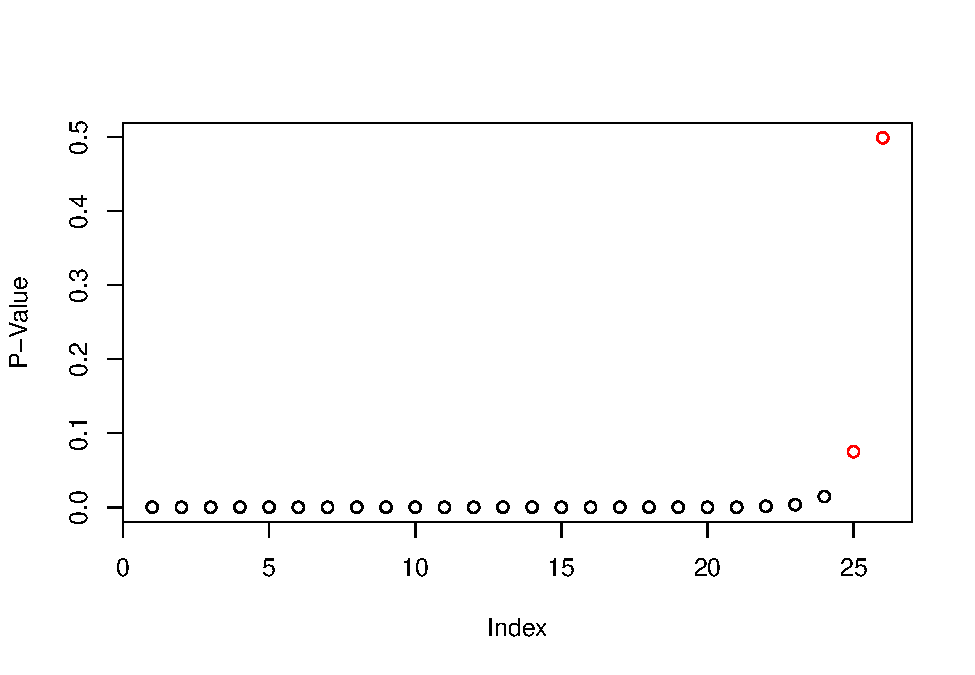
\includegraphics{dlassoMarkdown_files/figure-latex/unnamed-chunk-5-1.pdf}

\begin{Shaded}
\begin{Highlighting}[]
\NormalTok{noreject2 <-}\StringTok{ }\KeywordTok{which}\NormalTok{(noreject2)}
\NormalTok{p2 <-}\StringTok{ }\NormalTok{p2[noreject2,]   }\CommentTok{# these one's we cannot reject the null}
\KeywordTok{names}\NormalTok{(p2) <-}\StringTok{ }\KeywordTok{c}\NormalTok{(}\StringTok{"p-value"}\NormalTok{,}\StringTok{"Sig. Level"}\NormalTok{,}\StringTok{"BY Stat"}\NormalTok{)}
\NormalTok{p2}
\end{Highlighting}
\end{Shaded}

\begin{verbatim}
##                p-value Sig. Level    BY Stat
## DECADE1TRUE 0.07498765          . 0.02519782
## AGEP_HINS31 0.49921838            0.02594424
\end{verbatim}

\begin{Shaded}
\begin{Highlighting}[]
\CommentTok{# get BY-adjusted p-values}
\NormalTok{pBY2 <-}\StringTok{ }\KeywordTok{as.data.frame}\NormalTok{(}\KeywordTok{p.adjust}\NormalTok{(p2[,}\DecValTok{1}\NormalTok{], }\DataTypeTok{method =} \StringTok{"BY"}\NormalTok{))   }\CommentTok{#Benjamini-Yekutieli}
\KeywordTok{rownames}\NormalTok{(pBY2) <-}\StringTok{ }\KeywordTok{rownames}\NormalTok{(p2)}
\NormalTok{adjsigcode <-}\StringTok{ }\KeywordTok{cut}\NormalTok{(pBY2[,}\DecValTok{1}\NormalTok{], }\DataTypeTok{breaks =} \KeywordTok{c}\NormalTok{(}\OperatorTok{-}\OtherTok{Inf}\NormalTok{, }\FloatTok{0.001}\NormalTok{, }\FloatTok{0.01}\NormalTok{, }\FloatTok{0.05}\NormalTok{, }\FloatTok{0.1}\NormalTok{, }\DecValTok{1}\NormalTok{), }
                  \DataTypeTok{labels =} \KeywordTok{c}\NormalTok{(}\StringTok{"***"}\NormalTok{, }\StringTok{"**"}\NormalTok{, }\StringTok{"*"}\NormalTok{, }\StringTok{"."}\NormalTok{, }\StringTok{" "}\NormalTok{))}
\NormalTok{pBY2}\OperatorTok{$}\StringTok{""}\NormalTok{ <-}\StringTok{ }\NormalTok{adjsigcode}

\CommentTok{# compare p-values for non-rejected}
\NormalTok{fdr2 <-}\StringTok{ }\KeywordTok{cbind.data.frame}\NormalTok{(p2[,}\KeywordTok{c}\NormalTok{(}\DecValTok{1}\NormalTok{,}\DecValTok{2}\NormalTok{)], pBY2)}
\KeywordTok{colnames}\NormalTok{(fdr2) <-}\StringTok{ }\KeywordTok{c}\NormalTok{(}\StringTok{"Original"}\NormalTok{,}\StringTok{"Sig. Level"}\NormalTok{, }\StringTok{"FDR Adj."}\NormalTok{,}\StringTok{"Sig. Level"}\NormalTok{)}
\NormalTok{fdr2}
\end{Highlighting}
\end{Shaded}

\begin{verbatim}
##               Original Sig. Level  FDR Adj. Sig. Level
## DECADE1TRUE 0.07498765          . 0.2249630           
## AGEP_HINS31 0.49921838            0.7488276
\end{verbatim}

\end{document}
